% SIGGRAPH Asia 2026 Technical Papers (dual-track / Conference + Journal).
% Format per https://asia.siggraph.org/2026/submissions/technical-papers/
% Requires acmart.cls version 2.16 or newer (ACM Primary Article Template).
%
% Length policy: 7 pages excluding references and up to 2 figures-only pages.
% Detailed tables and dataset construction live in supplementary.tex; the main
% body links to them via xr-hyper (same submission bundle).
\documentclass[acmtog,anonymous,review]{acmart}

\citestyle{acmauthoryear}

%% Assigned submission ID from the Linklings form (placeholder).
\acmSubmissionID{0000}

\setcopyright{none}
\copyrightyear{2026}
\acmYear{2026}
\acmDOI{10.1145/nnnnnnn.nnnnnnn}
\acmJournal{TOG}
\acmVolume{45}
\acmNumber{6}
\acmArticle{1}
\acmMonth{12}

\received{12 May 2026}
\received[revised]{}
\received[accepted]{}

\usepackage{amsmath}
\usepackage{graphicx}
% Figures live in Paper/figures/. First path: latexmk from Paper/; second: cwd at repo root.
\graphicspath{{figures/}{Paper/figures/}}
\usepackage{booktabs}
% NB: do not load amssymb; acmart + newtxmath already define AMS symbols, and loading
% amssymb triggers "Command \Bbbk already defined" and aborts pdflatex.

% Cross-document \ref{} to labels in supplementary.tex (requires supplementary.aux;
% build with: latexmk supplementary.tex && latexmk paper.tex).
\usepackage{xr-hyper}
% Prefix required: both documents use acmart and share internal labels (e.g. tocindent-*).
\externaldocument[SX-]{supplementary}

\begin{document}

\title{Hierarchical Transformer Preconditioning for Interactive Physics Simulation}

\author{Anonymous Author(s)}
\affiliation{%
  \institution{Paper under double-blind review}
  \country{}}

\renewcommand{\shortauthors}{Anonymous Author(s)}

\begin{abstract}
Neural preconditioners promise data-driven priors for the linear systems that dominate
real-time physics simulation, but existing graph-neural designs struggle with long-range
couplings: their nonzero pattern is constrained to that of the system matrix, and information
between distant degrees of freedom must traverse many message-passing layers. We introduce a
neural preconditioner anchored to a weak-admissibility $\mathcal{H}$-matrix partition.
The partition is computed analytically and reused for all inputs, giving the network a strong
multiscale structural bias: a transformer stack handles dense diagonal blocks at full rank,
and a second stack emits low-rank factors for off-diagonal tiles at a single coarse resolution
regardless of tile size. Because every off-diagonal block is processed at the same token count,
the architecture's compute and memory scale linearly in problem size, $\Theta(N)$, rather than
the $O(N\log N)$ of classical $\mathcal{H}$-matrix arithmetic.
We train the preconditioner self-supervised with a cosine-similarity Hutchinson probe loss
that, unlike Frobenius-style objectives, is invariant to both the scale and the absolute
location of the eigenvalues of $MA$, letting the network cluster the spectrum wherever the
residual makes alignment easiest. At inference,
the entire PCG step (preconditioner application plus sparse matvec) is a sequence of batched
GEMMs over contiguous memory, with no triangular solves or data-dependent branching, captured
end-to-end in a single CUDA Graph.
On a stiff multiphase pressure-Poisson benchmark spanning $1\,024$--$16\,384$ unknowns and
density contrast ratios up to $100\!:\!1$, our preconditioner is the only method evaluated
that fits inside an interactive ($60$\,fps) budget across the entire range up to
$N\!=\!4\,096$, and it remains within a $24$\,fps budget at $N\!=\!16\,384$. At
$N\!=\!8\,192$, mean end-to-end solve time is $18.1\!\pm\!2.4$\,ms ($3.2$\,ms inference $+$
$14.9$\,ms PCG over $174$ iterations) versus $38.8\!\pm\!10.5$\,ms for GPU Jacobi,
$117.7\!\pm\!4.1$\,ms for AMGX classical AMG, and $449.6\!\pm\!83.7$\,ms for AMGX
\textsc{multicolor\_dilu}---a $2.1\times$ speedup over the best baseline that fits an
interactive budget and over $24\times$ over the best classical GPU preconditioner we evaluate.
\end{abstract}

\begin{CCSXML}
<ccs2012>
 <concept>
  <concept_id>10010147.10010341.10010342.10010343</concept_id>
  <concept_desc>Computing methodologies~Physical simulation</concept_desc>
  <concept_significance>500</concept_significance>
 </concept>
 <concept>
  <concept_id>10010147.10010257.10010293.10010294</concept_id>
  <concept_desc>Computing methodologies~Neural networks</concept_desc>
  <concept_significance>300</concept_significance>
 </concept>
</ccs2012>
\end{CCSXML}
\ccsdesc[500]{Computing methodologies~Physical simulation}
\ccsdesc[300]{Computing methodologies~Neural networks}

\keywords{preconditioning, iterative solvers, hierarchical matrices, transformers,
neural operators, physics simulation, real-time graphics}

\maketitle

% ===========================================================================
\section{Introduction}
\label{sec:intro}
% ===========================================================================

Real-time simulation of fluids, soft bodies, and coupled multiphysics systems often reduces,
at every time step, to solving a large sparse linear system $A\mathbf{x} = \mathbf{b}$ --
most commonly a symmetric positive-definite (SPD) pressure or stress system attacked with a
Krylov method such as preconditioned conjugate gradient (PCG)~\cite{saad2003iterative}. Many
simulation pipelines bypass this entirely (position-based dynamics, explicit SPH) or use
nonsymmetric Krylov variants and direct solvers, but for the SPD systems that dominate
incompressible-fluid and elastic-solid pipelines, PCG remains the workhorse. The
preconditioner $M\!\approx\!A^{-1}$ is the dominant design variable: it must be cheap to
apply and must cluster the eigenvalues of $MA$ tightly enough to drive PCG to its tolerance
in a few dozen iterations. Classical preconditioners --- Jacobi, incomplete Cholesky/LU
(IC/ILU)~\cite{lin1999incomplete}, sparse approximate inverses (SPAI)
\cite{kolotilina1993factorized,benzi1996sparse}, and algebraic multigrid
(AMG)~\cite{ruge1987algebraic} --- are well-understood and excel in many regimes,
particularly when the matrix is reused across many solves so a heavy setup amortizes. In an
interactive setting, however, $A$ changes at every frame, so any preconditioner whose setup
cost approaches the per-frame budget cannot amortize; this affects IC and AMG most because
their setup is sequential and irregular~\cite{naumov2015amgx}, and IC application is further
bottlenecked on triangular solves whose data hazards resist GPU
parallelization~\cite{liu2016synchronization,yamazaki2020performance}.

Machine learning offers an appealing alternative: given a distribution of simulation states,
a neural preconditioner can be trained once and amortized across frames at near-constant,
predictable inference cost. Graph neural networks (GNNs) have become the dominant
architecture for this purpose~\cite{Li2023learning,hausner2023neural,chen2024gnp,Yang2025sparse},
because the natural graph interpretation of a sparse matrix lets message-passing layers
propagate information through its nonzero pattern. However, this same choice imposes two
fundamental limitations that become acute in real-time simulation. First, GNN preconditioners
typically inherit the sparsity pattern of $A$ or of an incomplete factor of $A$: non-adjacent
interactions are either ignored entirely or only approximated through repeated graph
convolutions, which require many layers to propagate long-range information and tend to
oversmooth local detail along the way~\cite{chen2020simple,trifonov2025gnn}. Second, the
dominant operations at apply time---triangular solves on a learned IC factor, or sparse
matrix-vector products on a learned SPAI---are bandwidth-bound and either serialize on data
hazards~\cite{liu2016synchronization} or scatter through irregular memory access.

\paragraph{From PCG geometry to hierarchical structure.}
PCG's convergence rate is governed by the spectrum of $MA$, so the ideal preconditioner is
$M\!=\!A^{-1}$; any practical alternative trades approximation quality for cheapness of
representation and application. Although $A$ is sparse, $A^{-1}$ is generally dense, so the
relevant question is what \emph{structure} makes $A^{-1}$ cheap to store and apply
approximately. That structure is determined by the index ordering of $A$. In modern
simulation codes, degrees of freedom are commonly already arranged along a space-filling
curve (Morton/Z, Hilbert) or a bandwidth-reducing permutation (reverse Cuthill--McKee), not
because the linear solver wants it but because the surrounding pipeline does: spatial-hash
and BVH data structures used for neighbor search, broad-phase collision, and parallel
particle access build their indices from exactly these
orderings~\cite{karras2012maximizing,teschner2003optimized,ihmsen2011parallel}. Under such
orderings, the nonzeros of $A$ cluster near the main diagonal: near-diagonal entries describe
spatially local interactions, while far-diagonal entries, when they exist, describe distant
ones.

The corresponding inverse $A^{-1}$ is dense, but it inherits a softer form of this geometry:
sub-blocks of $A^{-1}$ associated with index ranges that are well-separated along the
ordering have rapidly decaying singular values, with the numerical rank shrinking as the
separation grows. \emph{Hierarchical matrices}, or
$\mathcal{H}$-matrices~\cite{hackbusch1999sparse,hackbusch2002adaptive,borm2003introduction},
are the data structure that exploits this prior: they represent $A$ or $A^{-1}$ as a
recursive partition into dense diagonal blocks plus low-rank off-diagonal blocks, with the
admissible rank shrinking as off-diagonal tiles move further from the main diagonal. The
fast multipole method (FMM)~\cite{greengard1987fast} exploits the same prior more
aggressively for translation-invariant kernels, factoring far-field interactions through
coarse low-dimensional surrogates; an $\mathcal{H}$-matrix preconditioner is, architecturally,
an FMM-shaped operator on the assembled system. Multigrid analysis~\cite{briggs2000multigrid}
relies on a related hierarchy, but interleaves smoothing with restriction/prolongation across
levels, whereas FMM and $\mathcal{H}$-matrix application has the flat one-pass structure
(coarse summary, far-field broadcast, local correction) that we adopt below.

\paragraph{Approach.}
We anchor the preconditioner to a weak-admissibility $\mathcal{H}$-matrix
partition~\cite{hackbusch2002adaptive}, computed analytically from the leaf-index geometry
and reused for every frame. With minimum block size $L$ and $K = N/L$ leaves, the partition
consists of $K$ dense diagonal blocks of size $L\!\times\!L$ (one per leaf) and a set of
off-diagonal tiles, each spanning $S\!\times\!S$ leaves with $S\!=\!2^{j}$, indexed by leaf
coordinates. A two-stream transformer operates on this layout: a
\emph{diagonal} stream emits one factor matrix per leaf at full rank, and an
\emph{off-diagonal} stream emits one factor matrix per tile at a constant coarse token count
$L_s\!=\!L/p$, regardless of $S$. The implied full-resolution block then has rank at most
$L_s$ on a $SL\!\times\!SL$ region, so the rank fraction $L_s/(SL)$ shrinks automatically as
$S$ grows---exactly the structural bias $\mathcal{H}$-matrix compression already calls for.
To break the locality of within-block attention without giving up the $\Theta(N)$ budget, we
route information between layers through \emph{highway} buffers organized as axial
(row/column-band) buffers and a single global summary token
(Section~\ref{sec:method:highways}).

\paragraph{A loss with no preferred eigenvalue location.}
We train this network self-supervised with a cosine-similarity Hutchinson probe loss on the
preconditioned image $MA\mathbf{z}$ of random probes $\mathbf{z}$. Compared to Frobenius- or
SAI-style objectives~\cite{Yang2025sparse}, the cosine objective is invariant to both the
scale and the absolute location of the eigenvalues of $MA$: it imposes no preferred location
or scale for the eigenvalue cluster, only that the preconditioned probe align angularly with
its source. The network is free to be \emph{lazy} -- to cluster the spectrum wherever doing
so minimizes the angular gap between $\mathbf{z}$ and $MA\mathbf{z}$ the most, without paying
for the wrong overall scale or center. This matters for stiff multiphase systems whose
spectra do not naturally cluster around $1$.

\paragraph{One CUDA Graph for the whole iteration.}
Every preceding choice -- analytically determined partition, fixed coarse rank, no
triangular solves, allocation-free apply -- cooperates to remove the data dependencies that
would normally fragment a CG iteration into separately dispatched kernels. The full PCG
inner loop -- preconditioner apply, sparse matvec, residual update, scalar reductions --
becomes a single fixed sequence of batched GEMMs and reductions over preallocated contiguous
tensors with no data-dependent branching. We capture it end-to-end as a single CUDA Graph
and replay it once per iteration, eliminating CPU dispatch overhead between every kernel of
every iteration. This is, in our measurements, the largest single source of the speedup we
report against classical GPU preconditioners.

\paragraph{Contributions.} (1) A neural preconditioner anchored to a weak-admissibility
$\mathcal{H}$-matrix partition, with a uniform-resolution off-diagonal stream that yields
$\Theta(N)$ inference and apply, in contrast to the $O(N\log N)$ of classical
$\mathcal{H}$-matrix arithmetic. (2) Multiscale highway connections that propagate axial and
global context between transformer layers without breaking the linear budget. (3) A
scale- and location-invariant cosine Hutchinson training objective that drops the implicit
eigenvalue-location prior of Frobenius- and SAI-style losses, letting the network choose
where in the spectrum to cluster $MA$. (4) An end-to-end allocation-free apply path that
captures into a single CUDA Graph, giving zero CPU dispatch overhead per PCG iteration.

% ===========================================================================
\section{Related Work}
\label{sec:related}
% ===========================================================================

\paragraph{Classical iterative solvers.}
Preconditioning sparse SPD systems is a textbook concern of scientific
computing~\cite{saad2003iterative}. The canonical algebraic preconditioners --- Jacobi,
incomplete Cholesky/LU (IC/ILU)~\cite{lin1999incomplete}, sparse approximate inverses
(SPAI)~\cite{kolotilina1993factorized,benzi1996sparse}, and algebraic multigrid
(AMG)~\cite{ruge1987algebraic} --- are mature, well-analyzed, and remain the default choice
across most of scientific computing. IC and ILU mirror the elimination structure of $A$
within a chosen sparsity pattern, giving strong spectral approximation per unit memory.
SPAI methods approximate $A^{-1}$ directly as a sparse matrix, exposing parallelism by
replacing triangular solves with a sparse matvec at apply time, with the choice of sparsity
pattern controlling the approximation/cost trade-off. AMG constructs a hierarchy of
coarsened operators algebraically and achieves near-optimal convergence on elliptic
problems~\cite{ruge1987algebraic,naumov2015amgx}. These methods are at their best when the
system is reused across many solves so a careful setup amortizes; the regime we target ---
$A$ changing every frame at interactive rates --- sits outside that comfort zone, which is
what motivates the amortized neural alternative pursued in this paper. The known GPU costs
of triangular solves~\cite{liu2016synchronization,yamazaki2020performance} and of AMG
setup/V-cycle communication~\cite{naumov2015amgx} bear directly on this regime rather than
on the methods themselves.

\paragraph{Neural operators and learned PDE solvers.}
Neural operators including Fourier-based~\cite{li2021fourier},
DeepONet-based~\cite{lu2021learning}, and graph-based~\cite{li2020neural,li2020multipole}
variants learn function-space mappings between coefficient and solution fields and
generalize across coefficient distributions, and have been deployed both as PDE surrogates
and as inner preconditioners for flexible Krylov solvers~\cite{rudikov2024neural}.
Physics-informed networks~\cite{raissi2019physics} embed PDE residuals directly into the
loss to enforce equation consistency without labeled solutions. Together these works
establish that neural networks can capture the global solution behavior of an operator
family from data; the present paper shares the broader ambition of replacing analytical work
with learned components, but operates one rung lower in the stack, on the assembled
algebraic system rather than the underlying PDE.

\paragraph{Learning-based preconditioners.}
A productive line of work trains GNNs to produce a learned incomplete factorization of $A$:
the network emits the nonzero values of a triangular factor on a chosen sparsity pattern,
replacing the heuristic fill-in and ordering choices of classical IC with a forward pass
trained on a distribution of matrices~\cite{Li2023learning,hausner2023neural,trifonov2024linear}.
Yang \emph{et al.}~\cite{Yang2025sparse} develop a complementary direction in which a GNN
emits a sparse approximate inverse in factored $GG^\top$ form, evaluated as two SpMVs at
apply time, and show that a scale-invariant Frobenius (``SAI'') loss enables effective
self-supervised training without ever forming a solution vector --- an idea our own
self-supervised objective builds on. Chen~\cite{chen2024gnp} reports strong performance
across the SuiteSparse collection on ill-conditioned problems where classical IC and AMG
struggle, demonstrating the breadth of the GNN preconditioner approach.
Trifonov~\emph{et al.}~\cite{trifonov2025gnn} analyze how local message passing relates to
the global elimination tree, clarifying when GNN architectures suffice for matrix-level
tasks. The present paper is in this lineage, and our point of departure is structural ---
described in the next section --- rather than a critique of the algorithmic choices these
works make.

\paragraph{Hierarchical neural architectures for PDEs.}
A parallel line of work embeds FMM- or $\mathcal{H}$-matrix-style hierarchical structure
directly into neural network architectures. $\mathcal{H}$-matrix-shaped multiscale
networks~\cite{Fan2019multiscale}, multipole graph neural operators~\cite{li2020multipole},
neural FMM/Green's-function operators~\cite{Fognini2025neural}, and neural-HSS
solvers~\cite{Sittoni2026neural} each demonstrate that hierarchical inductive biases let a
network represent long-range couplings without relying on fully connected attention or deep
stacks of purely local message passing. In a setting closer to ours, neural approximate
inverse preconditioners~\cite{Xu2025neural} and multigrid-inspired neural iterative
solvers~\cite{Lyu2026multigrid,Luz2020learning} use related structure to accelerate an
outer iteration. Collectively, this literature makes a strong case that an explicit
hierarchical/coarsening prior is a productive way to scale neural PDE machinery, and our
work adopts the same prior.

\paragraph{Hierarchical matrix techniques.}
Classical $\mathcal{H}$- and $\mathcal{H}^2$-matrix
arithmetic~\cite{hackbusch1999sparse,hackbusch2002adaptive,borm2003introduction} gives a
near-linear-cost framework for storing and applying operators whose well-separated
sub-blocks are low-rank, with mature machinery for adaptive partitioning, low-rank
truncation, and approximate factorization. HODLR variants~\cite{Hartland2023hodlr} apply the
same structural prior to dense Hessians in PDE-constrained inverse problems. The
partitioning machinery developed in this body of work is what we instantiate; the
contribution of the present paper lies in how the off-diagonal factors are produced and
applied, which is the subject of Section~\ref{sec:method}.

% ===========================================================================
\section{Background}
\label{sec:background}
% ===========================================================================

\paragraph{Conjugate gradient and the role of the spectrum.}
Given an SPD system $A\mathbf{x}=\mathbf{b}$, the conjugate gradient
method~\cite{saad2003iterative} produces at iteration $k$ the unique vector $\mathbf{x}_k$ in
the Krylov subspace $\mathcal{K}_k(A,\mathbf{r}_0) = \mathrm{span}\{\mathbf{r}_0, A\mathbf{r}_0,
\ldots, A^{k-1}\mathbf{r}_0\}$ that minimizes the energy norm $\|\mathbf{x}_k -
\mathbf{x}^*\|_A$. Equivalently, the error $\mathbf{e}_k$ satisfies
\begin{equation}
  \|\mathbf{e}_k\|_A \;=\; \min_{p\in\mathcal{P}_k,\,p(0)=1}\;\|p(A)\,\mathbf{e}_0\|_A
  \;\le\; \mathbf{e}_0\,\max_{\lambda\in\sigma(A)}|p(\lambda)|,
  \label{eq:cg-poly}
\end{equation}
where $\mathcal{P}_k$ is the space of degree-$k$ polynomials and $\sigma(A)$ is the spectrum.
Because $p(A)$ acts diagonally in the eigenbasis of $A$, CG's progress is dictated entirely
by how small a degree-$k$ polynomial with $p(0)=1$ can be made on the eigenvalues of $A$. Two
consequences of \eqref{eq:cg-poly} shape preconditioner design.

First, the textbook condition-number bound
$\|\mathbf{e}_k\|_A \le 2\bigl((\sqrt{\kappa}-1)/(\sqrt{\kappa}+1)\bigr)^k \|\mathbf{e}_0\|_A$,
with $\kappa=\lambda_{\max}/\lambda_{\min}$, follows from the Chebyshev polynomial on the
interval $[\lambda_{\min},\lambda_{\max}]$ and is tight only when the spectrum actually fills
that interval. In practice, the \emph{distribution} of eigenvalues within
$[\lambda_{\min},\lambda_{\max}]$ matters at least as much as the ratio.

Second, the polynomial in \eqref{eq:cg-poly} can place its $k$ roots wherever the spectrum
concentrates. If $\sigma(A)$ collapses to $c$ tight clusters, a degree-$c$ polynomial that
vanishes once on each cluster drives the error to roughly the cluster widths, so CG converges
in $\sim c$ iterations in exact arithmetic regardless of how far apart the clusters are: two
or three well-separated tight clusters are no worse than one. By the same token, isolated
outlying eigenvalues (a few stiff modes from boundary conditions or material contrast) cost
only one extra iteration each, since one root of $p$ disposes of each outlier.

Preconditioning replaces $A\mathbf{x}=\mathbf{b}$ with $MA\mathbf{x}=M\mathbf{b}$ (left
preconditioning), and the same analysis applies to $\sigma(MA)$. The objective is therefore
not ``make $MA$ close to $I$ in any matrix norm'' but rather ``make $\sigma(MA)$ look like a
small number of tight clusters bounded away from zero,'' with the absolute scale and location
of those clusters largely irrelevant.

\paragraph{Hierarchical matrices.}
A hierarchical matrix ($\mathcal{H}$-matrix)~\cite{hackbusch1999sparse,hackbusch2002adaptive,borm2003introduction}
is a data-sparse representation of a dense matrix as a recursive block partition in which
each block is either small enough to store densely or has its singular values decay fast
enough to be stored as a low-rank factorization $UV^\top$. The construction has two
ingredients.

A \emph{cluster tree} recursively partitions the row/column index set $\{0,\ldots,N-1\}$
into nested subsets down to leaves of bounded size. A \emph{block cluster tree} then
enumerates pairs of index clusters $(\mathcal{I},\mathcal{J})$ and tags each pair as
\emph{admissible} (replaceable by a low-rank factor) or \emph{inadmissible} (kept dense).
The \emph{strong admissibility condition} of Hackbusch \emph{et al.}~\cite{hackbusch1999sparse}
requires geometric separation,
$\min\{\mathrm{diam}(\mathcal{I}),\mathrm{diam}(\mathcal{J})\}
\le \eta\,\mathrm{dist}(\mathcal{I},\mathcal{J})$,
and yields a fine partition that admits aggressive compression but contains many small
blocks. The \emph{weak admissibility condition}~\cite{hackbusch2002adaptive}, used in this
paper, requires only $\mathcal{I}\ne\mathcal{J}$ (or, in index-space form,
$|\mathcal{I}|\le\eta\,\mathrm{dist}(\mathcal{I},\mathcal{J})$ as in
HODLR~\cite{Hartland2023hodlr}), producing a coarser partition with larger but fewer
off-diagonal blocks --- a trade-off favorable for GPU batching.

The structural justification for low-rank approximation on admissible blocks is asymptotic
smoothness of the underlying kernel: for a Green's function $G(x,y)$ smooth away from $x=y$,
a truncated Taylor expansion on $\mathcal{I}\times\mathcal{J}$ achieves accuracy
$\varepsilon$ at rank $O(\log^d \varepsilon^{-1})$ independent of block size, and the same
exponential singular-value decay is observed empirically on inverses of discretized elliptic
operators. Classical $\mathcal{H}$-matrix arithmetic (mat-vec, addition, factorization, even
inversion) runs in $O(N\log N)$ to $O(N\log^2 N)$ time, with $\mathcal{H}^2$-matrices and
HSS variants reducing this further by also nesting the low-rank bases across levels.

\paragraph{Hutchinson trace estimation and probe spectra.}
For any matrix $B\in\mathbb{R}^{N\times N}$ and any random probe $\mathbf{z}\in\mathbb{R}^N$
with $\mathbb{E}[\mathbf{z}\mathbf{z}^\top]=I$, the Hutchinson
identity~\cite{hutchinson1989stochastic} gives
\begin{equation}
  \mathbb{E}_{\mathbf{z}}\bigl[\mathbf{z}^\top B \mathbf{z}\bigr]
  \;=\; \operatorname{tr}(B),
  \label{eq:hutch}
\end{equation}
an unbiased Monte Carlo estimate of $\operatorname{tr}(B)$ obtainable from one matrix-vector
product $B\mathbf{z}$ per probe, without ever materializing $B$. Standard probe distributions
include $\mathbf{z}\sim\mathcal{N}(0,I)$ and Rademacher $\mathbf{z}\in\{\pm 1\}^N$; the
former trades slightly higher variance for rotational invariance.

What matters for our subsequent use of these probes inside a learning objective --- as
opposed to as a pure trace estimator --- is their spectral content. Decompose $\mathbf{z}$
in the eigenbasis $\{\mathbf{u}_i\}$ of $B$:
$\mathbf{z} = \sum_i \alpha_i\,\mathbf{u}_i$, with $\alpha_i = \mathbf{u}_i^\top\mathbf{z}$.
For any isotropic probe distribution, $\mathbb{E}[\alpha_i^2]=1$ for every $i$: the probe
places equal expected energy on every eigenmode of $B$. Any scalar functional of
$(\mathbf{z}, B\mathbf{z})$ is therefore an unbiased measurement of $B$'s action across the
\emph{whole} spectrum, weighted uniformly --- it is not biased toward smooth/low-frequency or
oscillatory/high-frequency modes the way a probe drawn from a band-limited distribution
would be. This \emph{spectral whiteness} of isotropic probes is what allows a single scalar
loss built from $\mathbf{z}$ and $(MA)\mathbf{z}$ to faithfully reflect global preconditioner
quality across the entire spectrum of $MA$, and it is the property our training objective
relies on.

% ===========================================================================
\section{Method}
\label{sec:method}
% ===========================================================================

\paragraph{Notation.}
Throughout this section, $A\in\mathbb{R}^{N\times N}$ is the assembled sparse SPD system,
with degrees of freedom indexed along a space-filling-curve or bandwidth-reducing ordering.
The $N$ indices are partitioned into $K=N/L$ contiguous \emph{leaves} of size $L$; this
induces an $\mathcal{H}$-matrix partition consisting of $K$ diagonal leaf blocks and
$M_\mathcal{H}$ unique weakly-admissible \emph{off-diagonal tiles}, with tile $m$ spanning
$S_m\!\times\!S_m$ leaves (so covering an $S_mL\!\times\!S_mL$ region of $A$). The network
operates at channel width $d$ and uses $n_l$ transformer layers per attention stack. The
diagonal stream operates at full per-node resolution $L$ per leaf; the off-diagonal stream
operates at a coarse token count $L_s\!\ll\!L$ per tile. We use
$L\!=\!128,\,L_s\!=\!32,\,d\!=\!128,\,n_l\!=\!3$ in every reported result; the analysis
generalizes verbatim to other choices.

\paragraph{Pipeline and dispatch budget.}
The network is a four-stage pipeline from the simulation state and $A$ to a packed tensor of
factor matrices encoding an $\mathcal{H}$-matrix approximate inverse $M\!\approx\!A^{-1}$:
(1) a \emph{physics-aware encoder} (Sec.~\ref{sec:method:encoder}) lifts per-node and
per-edge features to width-$d$ node embeddings; (2) a \emph{diagonal attention stack}
(Sec.~\ref{sec:method:diag}) processes leaf-grouped tokens and emits one dense factor per
leaf; (3) an \emph{off-diagonal attention stack} (Sec.~\ref{sec:method:offdiag}) processes
tile-grouped tokens and emits one low-rank factor per off-diagonal tile; (4) linear decoder
heads (Sec.~\ref{sec:method:decoder}) produce the final factor tensors. \emph{There are
exactly two attention computations in the entire network} --- one batched over all $K$
leaves and one batched over all $M_\mathcal{H}$ tiles --- so a forward pass dispatches
exactly two attention kernels, independent of $N$. Combined with the static partition and
the absence of data-dependent branching elsewhere, this is what later lets training and PCG
inference run inside a single CUDA Graph.

\begin{figure}[t]
  \centering
  \begin{minipage}[t]{0.49\linewidth}
    \centering
    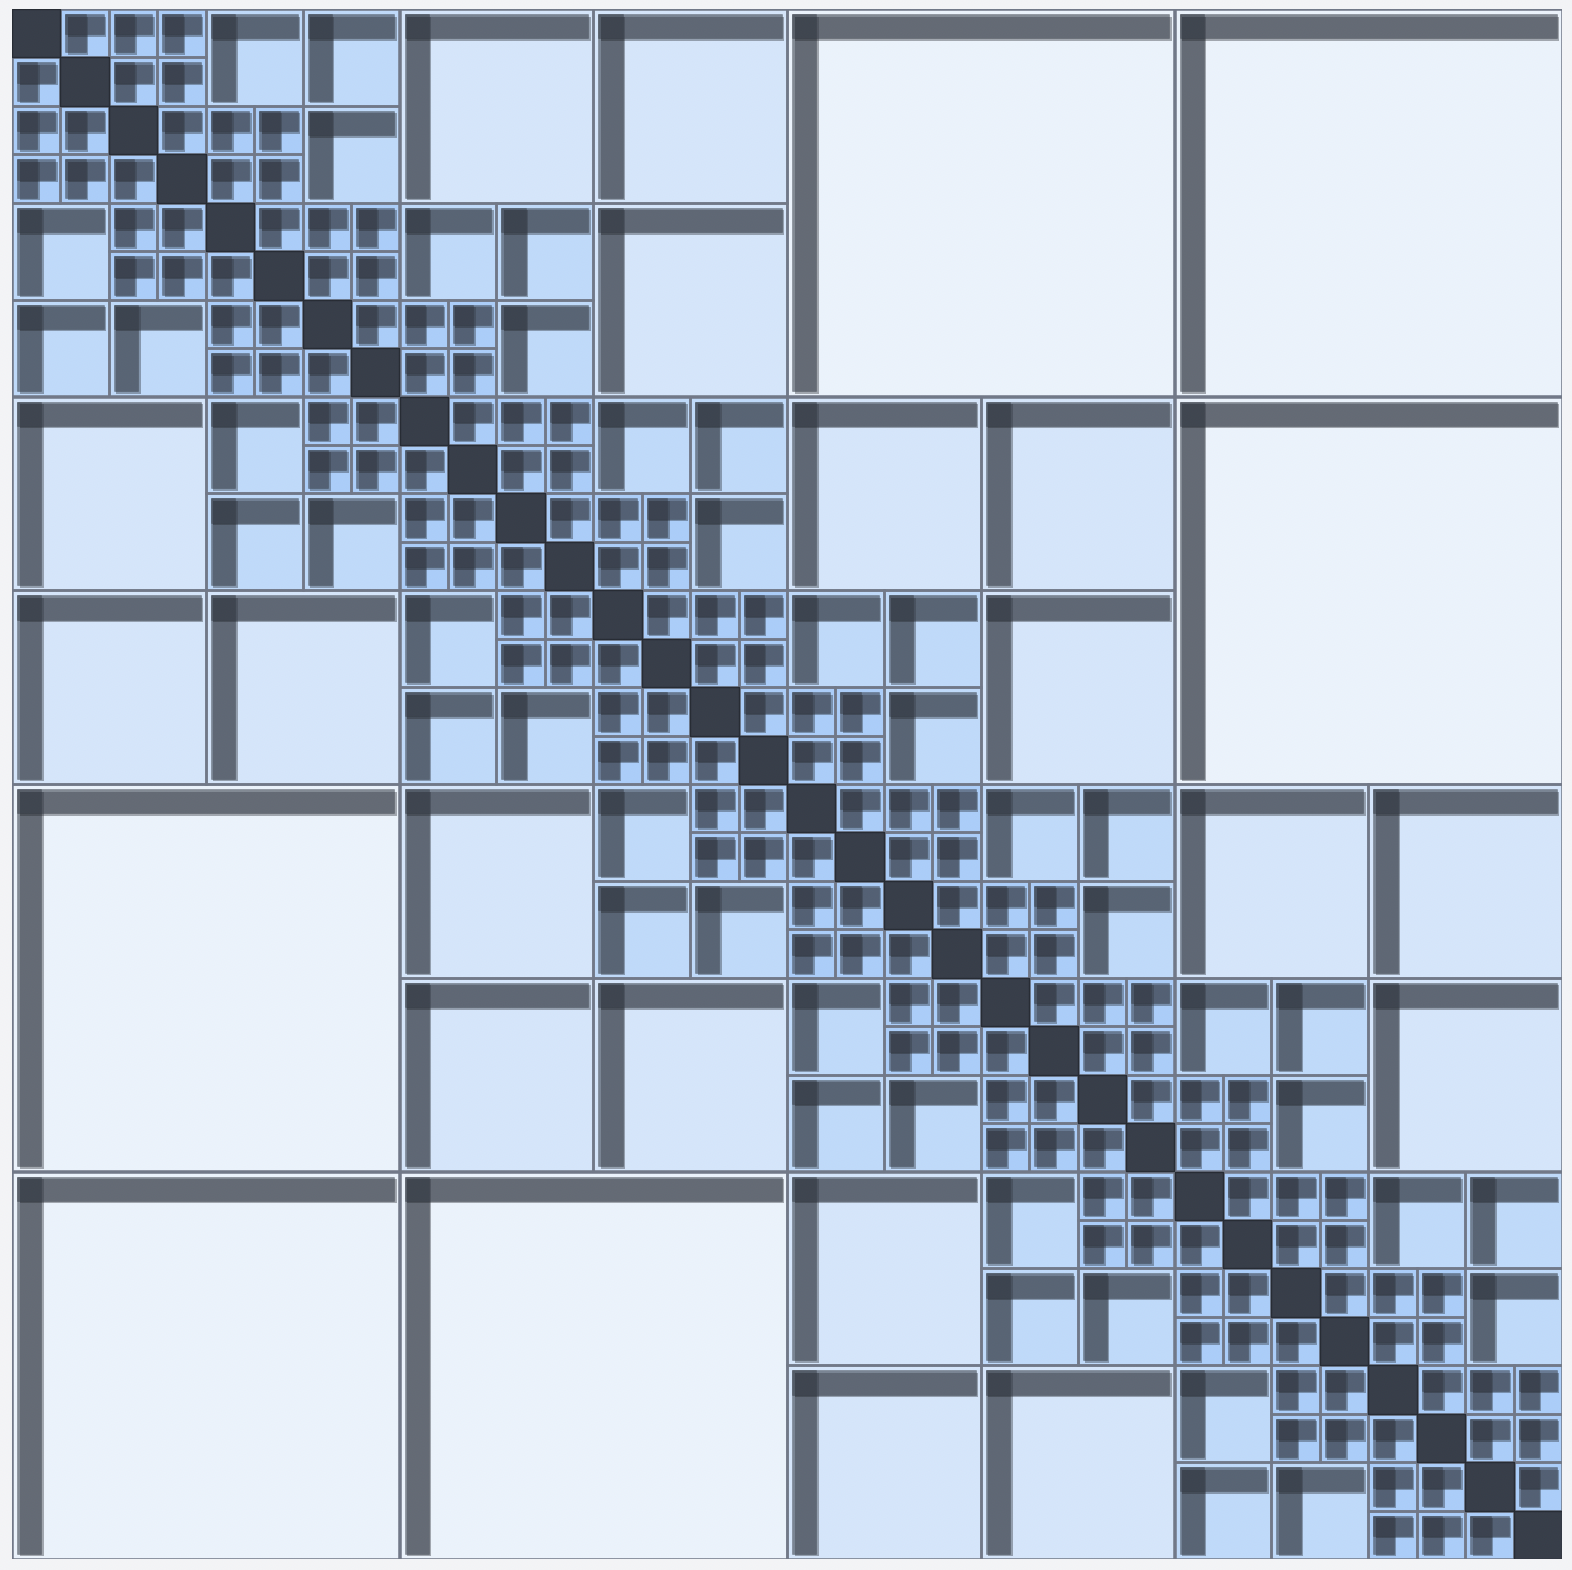
\includegraphics[width=\linewidth]{hmatrixgraphic.png}\\
    \small (a) $\mathcal{H}$-matrix partition.
  \end{minipage}\hfill
  \begin{minipage}[t]{0.49\linewidth}
    \centering
    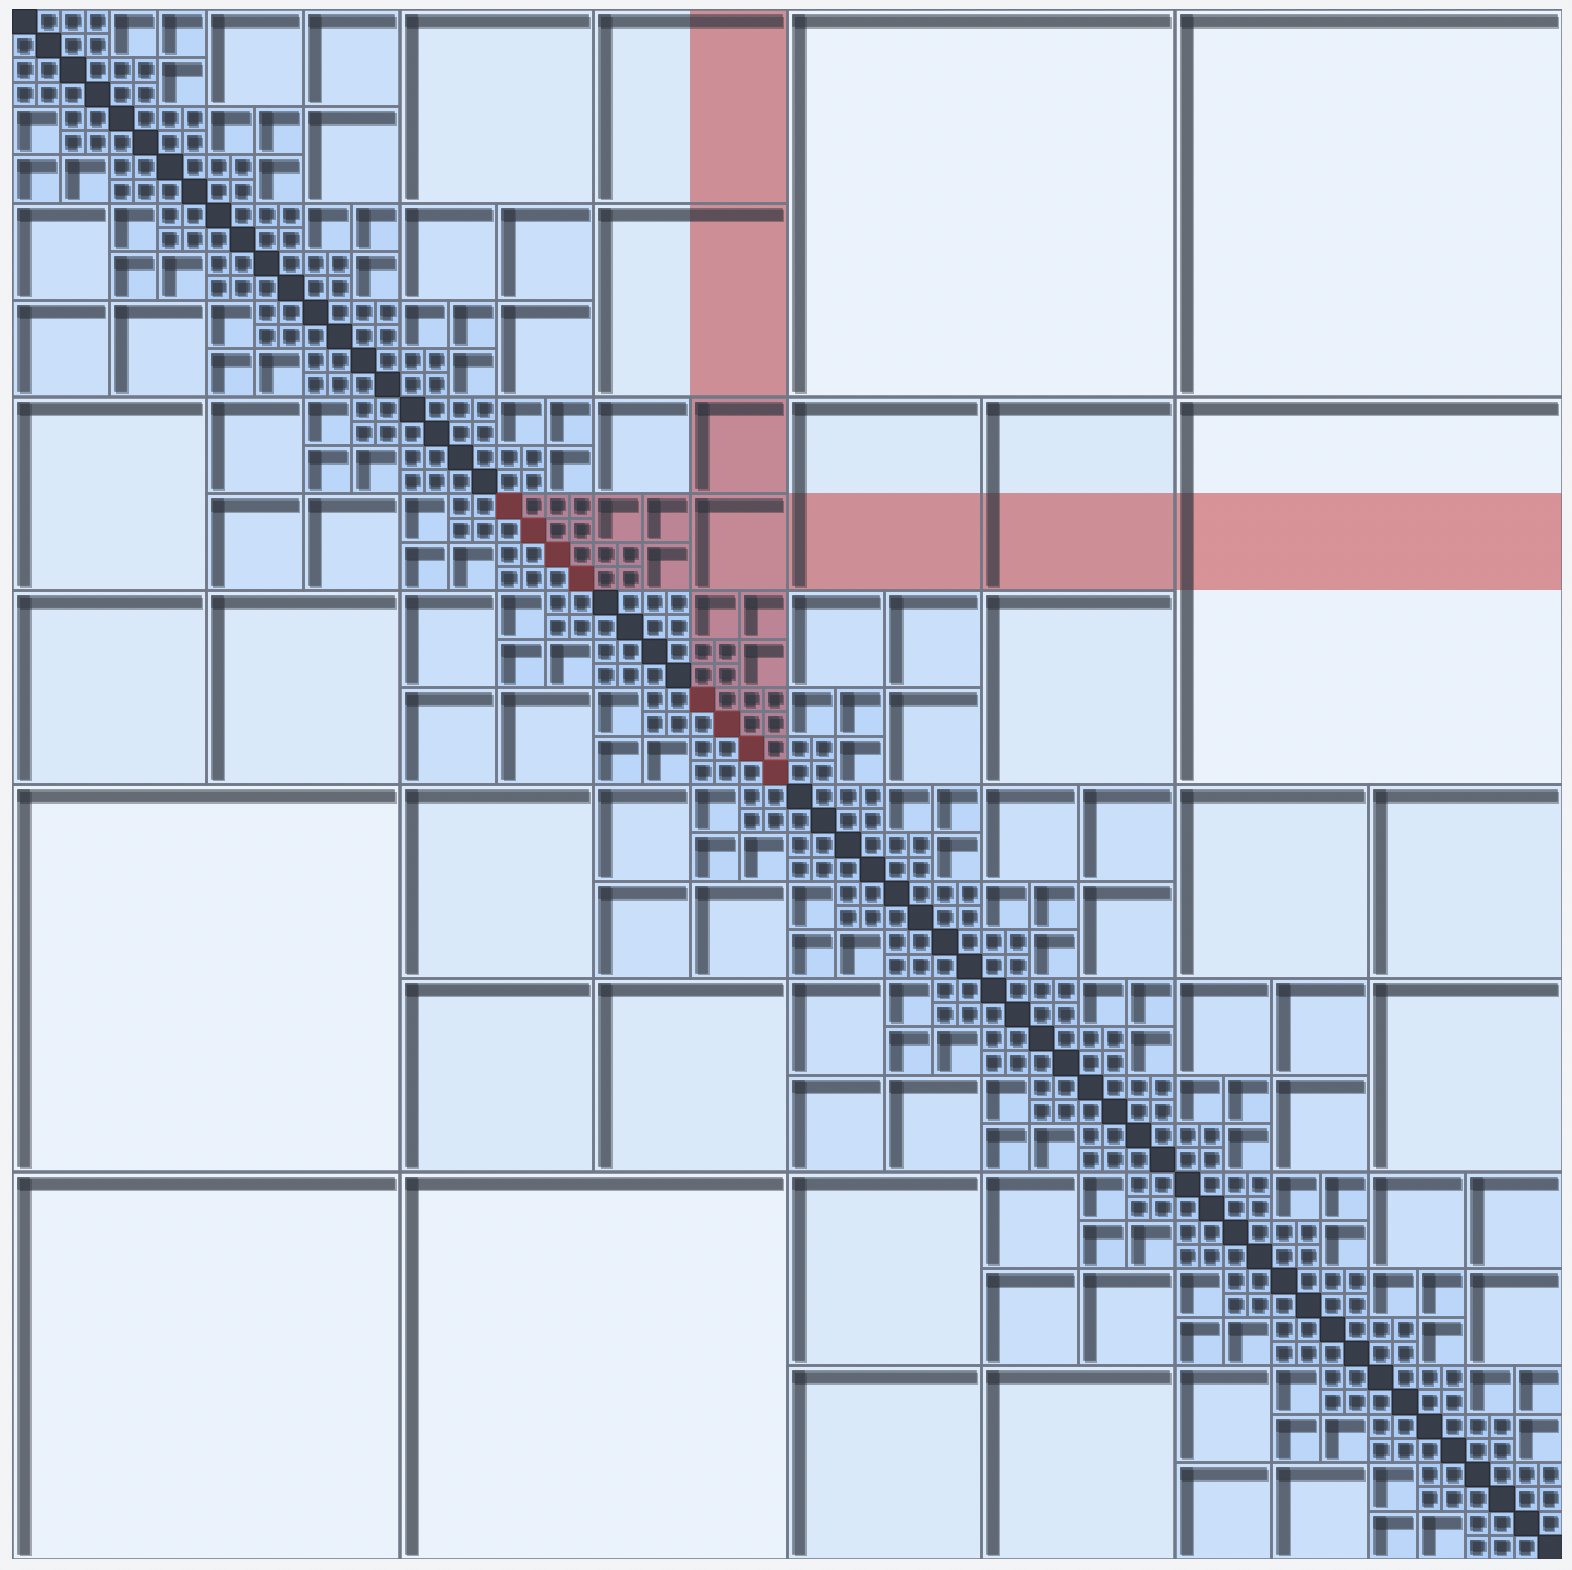
\includegraphics[width=\linewidth]{highwaysgraphic.png}\\
    \small (b) Highway channels.
  \end{minipage}
  \caption{Left: weak-admissibility $\mathcal{H}$-matrix partition. Dense diagonal leaf
    blocks lie along the main diagonal; admissible off-diagonal tiles double in size with
    separation from the diagonal. Translucent red overlays the row- and column-index sets of
    one exemplar tile. Right: per-layer communication channels added by the highway
    connections (Sec.~\ref{sec:method:highways}). The same off-diagonal tile contributes
    scatter-add updates to its row- and column-strip ranges in the axial highway buffers
    (translucent red), and to a single broadcast global token. Together with within-block
    attention these give the network four communication channels of dimensions
    $2\mathrm{D}/1\mathrm{D}/1\mathrm{D}/0\mathrm{D}$ per layer.}
  \label{fig:partition-and-highways}
\end{figure}

\subsection{From simulation state to per-node embeddings}
\label{sec:method:encoder}

Because the preconditioner is neural rather than algebraic, the network is not constrained
to ingest only the scalar entries $A_{ij}$: it can directly observe the per-node and
per-pair quantities that the simulator assembles into those entries, recovering information
that a fixed analytical preconditioner would never see. The encoder takes as input whichever
per-node features the simulator already exposes --- typically a subset of position,
velocity, density, pressure, temperature, and material parameters --- together with the
geometric and coupling features $(\Delta\mathbf{x}_{ij}, A_{ij})$ for every nonzero of $A$.
A two-layer MLP lifts the node features (optionally concatenated with a broadcast global
context vector) to dimension $d$, and $n_{\mathrm{gcn}}\!=\!2$ residual
graph-convolutional layers~\cite{kipf2017semi} mix in neighborhood information using $A$ as
the message-passing weight, yielding one width-$d$ embedding per node aware of its local
matrix entries and the physical state of its neighbors. This is the only stage of the
network that observes individual graph edges; everything downstream operates on the block
layout of the partition, decoupling cost from edge count.

\subsection{Diagonal attention stack}
\label{sec:method:diag}

For each of the $K$ leaves, the diagonal stack produces a square factor
$F_k\!\in\!\mathbb{R}^{L\times L}$, with the corresponding diagonal block of $M$ given by the
PSD outer product $F_kF_k^\top$. The encoder embeddings inside a leaf are processed at full
per-node resolution by $n_l$ transformer layers~\cite{Liu2021swin,vaswani2017attention} that
restrict attention to within the leaf --- the within-window attention pattern of Swin
adapted to one-dimensional index ranges. Attention logits carry a per-head bias produced by
a small MLP from the four-dimensional edge descriptor
$(\Delta\mathbf{x}_{ij}, A_{ij})$ for each in-leaf token pair, so geometry and coupling
strength can modulate attention directly. This is the first of the two attention dispatches
mentioned above; it is batched over all $K$ leaves.

\subsection{Off-diagonal attention stack}
\label{sec:method:offdiag}

For each off-diagonal tile $m$ spanning row index set $\mathcal{I}_m$ and column index set
$\mathcal{J}_m$ of size $S_mL$, the off-diagonal stack produces a pair of thin factor
matrices $U_m, V_m\!\in\!\mathbb{R}^{L_s\times L_s}$ whose outer product
$B_m\!=\!U_mV_m^\top$ is the tile's coarse-resolution representation. Two design choices
shape this stream.

\emph{Constant coarse token count, independent of tile size.} Per-node embeddings are pooled
along the row-strip $\mathcal{I}_m$ and the column-strip $\mathcal{J}_m$ of the encoder
output, then condensed along the in-strip axis to $L_s\!=\!L/p_{\mathrm{off}}$ tokens. Every
tile therefore arrives at the attention stack with the same shape $(L_s, d)$, regardless of
its physical size $S_mL$ --- a $4\times$ in-strip condensation for the smallest tiles and a
$S_m\!\cdot\!4\times$ condensation for the largest. Attention then runs across the $L_s$
tokens of each tile, batched over all tiles; this is the second (and final) attention
dispatch. Edge biases for each in-tile token pair are computed from the mean of
$(\Delta\mathbf{x}_{ij}, A_{ij})$ over all node pairs spanning the corresponding
row/column sub-strips.

\emph{Constant per-tile rank, hence shrinking rank fraction with separation.} The factor
pair $(U_m, V_m)$ has rank at most $L_s$, while the physical block it represents has size
$S_mL\!\times\!S_mL$; the rank fraction $L_s / (S_mL)$ decreases automatically as $S_m$
grows. This is the structural prior that makes $\mathcal{H}$-matrix compression effective:
distant tiles, encoding smoother long-range couplings, are compressed more aggressively than
near ones, while diagonal blocks remain at full rank (Sec.~\ref{sec:method:diag}). This
distribution of representation capacity --- dense local, low-rank far --- is precisely the
asymptotic-smoothness pattern documented for inverses of discretized elliptic operators
(Sec.~\ref{sec:background}).

Quantitatively, the constant rank $L_s\!=\!32$ is more than sufficient for the problem class
we target. Figure~\ref{fig:rank-headroom} compares it to the numerical rank required to
capture the corresponding tile of $A^{-1}$ at three truncation tolerances; even at
$\varepsilon\!=\!10^{-9}$, the provided rank exceeds the required rank by $2.6\times$ at the
largest tile size, with the gap widening as separation grows.

\begin{figure}[t]
  \centering
  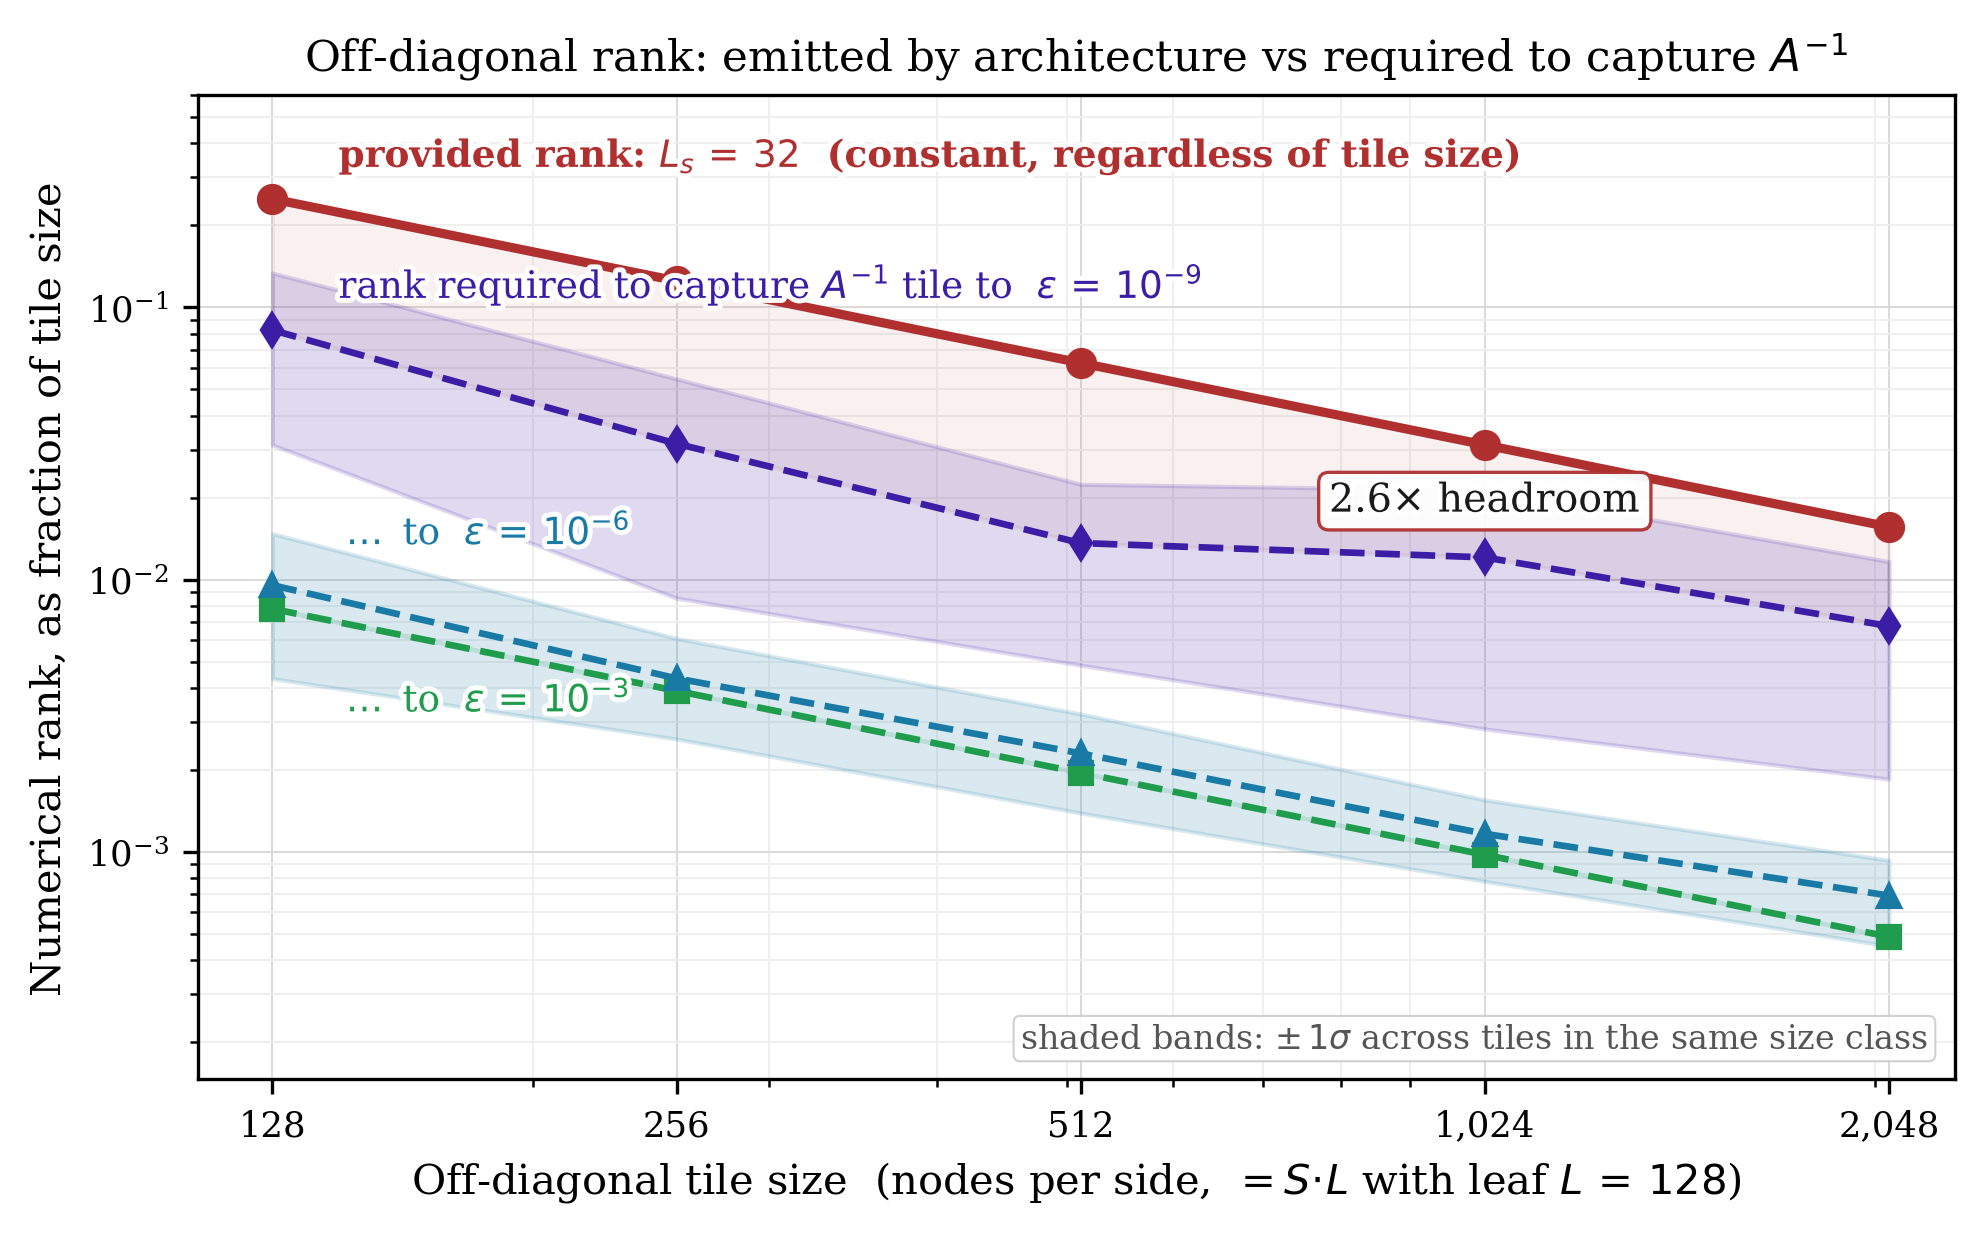
\includegraphics[width=0.85\linewidth]{rank_provided_vs_needed.png}
  \caption{Off-diagonal rank emitted by the architecture (constant $L_s\!=\!32$, red)
    versus numerical rank required to capture the corresponding tile of $A^{-1}$ to
    relative error $\varepsilon\!\in\!\{10^{-3},10^{-6},10^{-9}\}$ (dashed), reported as
    a fraction of tile size on \textsf{multiphase\_v2} frames with leaf $L\!=\!128$.
    Shaded bands: $\pm 1\sigma$ across tiles in the same size class. The provided rank
    sits above the required rank at every tile size and every tolerance, with
    $2.6\times$ headroom at the largest tile under the strictest tolerance.}
  \label{fig:rank-headroom}
\end{figure}

\paragraph{What happens as $N$ grows.}
A natural concern is whether a constant per-tile rank $L_s$ remains adequate as $N$ grows.
Two regimes are distinguished. (i) \emph{Larger simulations at fixed resolution.} If $N$
grows because the simulation domain grows --- more particles, more cells, the same physical
length scales and the same local interaction radius --- the partition simply contains more
tiles of the same maximum size, the singular-value decay rate of each tile is unchanged, and
the per-tile rank budget stays appropriate. This is the regime our experiments target.
(ii) \emph{Finer simulations at fixed domain.} If instead $N$ grows because the
discretization is refined, the largest tile size $S_{\max}L$ grows with it and the numerical
rank required for a fixed tolerance grows logarithmically with $S_{\max}$ for smooth
Green's functions (Sec.~\ref{sec:background}). Because $L$ and $p_{\mathrm{off}}$ are
hyperparameters, the natural response is to target a constant number of leaves $K$ rather
than a constant $L$; this scales $L$ with the domain dimension at the cost of a single
$O(N\log N)$ pooling pass and otherwise leaves the architecture untouched. We do not pursue
this in our experiments since the regime we evaluate does not span a discretization-refinement
octave wide enough to require it.

\subsection{Highway connections}
\label{sec:method:highways}

Within-leaf and within-tile attention build rich local representations but cannot directly
observe the global state. Highway connections restore this by coupling the diagonal and
off-diagonal stacks through three buffers maintained per transformer layer: row and column
\emph{axial} buffers
$\mathbf{r}_{\mathrm{hw}},\mathbf{c}_{\mathrm{hw}}\!\in\!\mathbb{R}^{B\times N\times d}$,
and a single global summary token
$\mathbf{g}_{\mathrm{hw}}\!\in\!\mathbb{R}^{B\times d}$ (illustrated in
Fig.~\ref{fig:partition-and-highways}b).

After the attention sublayer of each transformer block, block-token embeddings are
scatter-added into their corresponding rows of the axial buffers (off-diagonal tile tokens
are first repeat-interleaved back to full leaf resolution so each tile contributes uniformly
across its $S$-leaf row and column ranges), and the global token is then updated as the mean
over all active tokens. Before the FFN sublayer, each token concatenates its row, column,
and global highway context with its own embedding and feeds the resulting $4d$-wide vector
to the FFN's input projection. The four channels in each layer --- intra-block attention
(2D, local), row and column highways (1D, axial), and the global token (0D, broadcast) ---
compose a multiscale communication structure that mirrors the band-row-column-global
geometry of the inverse of a banded matrix. The highway adds one $O(Nd)$ scatter-gather per
layer, preserving overall $\Theta(N)$ scaling. Highways are enabled in every result we
report; we ablate the choice of channels in Section~\ref{sec:ablation}.

\subsection{Decoder, output, and the geometric picture}
\label{sec:method:decoder}

After both attention stacks, three lightweight decoder heads project token embeddings to
preconditioner factors:
\begin{itemize}
\item A \emph{leaf head} maps each diagonal-stream token (one per node, $L$ per leaf) through
a two-layer MLP and reshapes the result into a per-leaf factor
$F_k\!\in\!\mathbb{R}^{L\times L}$. The corresponding diagonal block of $M$ is
$F_kF_k^\top\!\in\!\mathbb{R}^{L\times L}$, PSD by construction.
\item Two \emph{off-diagonal heads} map each off-diagonal-stream token (one per coarse
position, $L_s$ per tile) linearly to $L_s$ output channels, yielding factor pairs
$U_m,V_m\!\in\!\mathbb{R}^{L_s\times L_s}$.
\item Two \emph{node heads} project the per-node diagonal-stream embeddings linearly to
$L_s$ output channels, producing per-leaf bridge matrices
$\tilde U_k,\tilde V_k\!\in\!\mathbb{R}^{L\times L_s}$ that connect the fine node-level
representation to the coarse tile-level representation.
\end{itemize}

\emph{Geometric picture.} The bridge and tile factors together implement an FMM-style
strip-to-strip chain (worked out in detail in Sec.~\ref{sec:application}). Reading along
the off-diagonal contribution to $M\mathbf{r}$ for a single tile: a residual $\mathbf{r}$
restricted to the column-strip $\mathcal{J}_m$ (length $S_mL$) is first contracted along the
strip by the per-leaf bridge $\tilde U_k^\top$ to produce coarse leaf summaries (length
$L_s$ per leaf in $\mathcal{J}_m$); these are then mixed across the tile by the
$L_s\!\times\!L_s$ factor $B_m\!=\!U_mV_m^\top$; and finally expanded back to full
node-resolution on the row-strip $\mathcal{I}_m$ by the per-leaf prolongation
$\tilde V_l$. The shape progression is therefore
\[
  \underbrace{S_mL}_{\text{strip}}
  \;\xrightarrow{\,\tilde U^\top\,}\;
  \underbrace{S_mL_s}_{\text{thinner strip}}
  \;\xrightarrow{\,B_m\,}\;
  \underbrace{S_mL_s}_{\text{thinner strip}}
  \;\xrightarrow{\,\tilde V\,}\;
  \underbrace{S_mL}_{\text{strip}},
\]
a fine strip that contracts to a coarse strip, transmits the coarse far-field interaction,
and re-expands to a fine strip. The geometry mirrors the FMM upward-pass / interaction-list /
downward-pass structure.

\emph{Positive-definiteness.}
By construction the diagonal contribution $\sum_k F_kF_k^\top$ is PSD. The full $M$ adds
indefinite low-rank off-diagonal corrections; in our experiments this assembled $M$ has
remained empirically PSD on every test system and PCG has never broken down on the
preconditioned system. Strict SPD enforcement is cheap if it should ever be needed: a
positive diagonal of $F_k$ (via elementwise softplus or exponential, the standard trick used
in prior neural ICs~\cite{Li2023learning,hausner2023neural}), together with a
diagonal-dominant scaling of off-diagonal factors, would guarantee strict positive
definiteness with negligible overhead. We do not enable these in our reported results.

\emph{Jacobi residual.} A scalar gate produces a per-node correction $\lambda_i$ added to
$\mathrm{diag}(\boldsymbol\lambda)\,\mathrm{diag}(A)^{-1}$. Early in training, when the
hierarchical factors approximate $A^{-1}$ poorly, this Jacobi residual provides a cheap
gradient sink that prevents loss stagnation; once the hierarchical factors are useful, the
gate's contribution tends to zero and capacity shifts to the structured branch.

All factors are concatenated into a single packed tensor of width
$P = K L^2 + M_\mathcal{H} L_s^2 + 2NL_s + N$, which is what the apply routine consumes.

\subsection{Complexity}
\label{sec:method:complexity}

Encoder cost is $O(Nd^2)$ for bounded-degree graphs. The diagonal attention stack processes
$K$ leaves of $L$ tokens each through $n_l$ layers: $O(n_l K L^2 d) = O(n_l N L d)$, linear
in $N$ at fixed $L,d,n_l$. The off-diagonal stack processes $M_\mathcal{H}\!=\!O(K)$ tiles of
$L_s$ tokens each: $O(n_l K L_s^2 d) = O(n_l N L_s^2 d / L)$, also linear in $N$. Highway
scatter-gather contributes $O(Nd)$ per layer. The total inference budget is therefore
$\Theta(N)$, with constants determined entirely by the fixed hyperparameters
$L, L_s, d, n_l$.

\paragraph{Measured breakdown.}
Profiling the forward pass at $N\!=\!8\,192$: attention stacks $\sim\!59\%$ (diagonal
$\sim\!36\%$, off-diagonal $\sim\!23\%$), encoder $\sim\!16\%$, decoder heads
$\sim\!18\%$, layout helpers $<\!4\%$. Only the attention portion scales with $n_l$, so the
transformer share rises toward $\sim\!75\%$ at the $n_l\!=\!3$ default. At the kernel
level, CUTLASS Tensor-Op GEMMs (\texttt{cutlass\_80\_tensorop\_s1688gemm} and
\texttt{sm90\_xmma\_gemm} TF32) consume $\sim\!31\%$ of device time and CUTLASS fused
attention (\texttt{fmha\_cutlassF}) a further $\sim\!14\%$, confirming that the hot path
dispatches to compute-bound Tensor Core kernels rather than to bandwidth-bound SpMV or
indexed-gather; the remainder is copies/reshapes and elementwise/normalization
($\sim\!17\%$ each).

% ===========================================================================
\section{Preconditioner Application}
\label{sec:application}
% ===========================================================================

PCG calls $M$ on the residual once per iteration. Two design choices keep this hot path
allocation-free, branch-free, and dispatchable as a single CUDA Graph. First, $M$ is never
formed explicitly: at full resolution its off-diagonal blocks reach
$\tfrac{N}{2}\!\times\!\tfrac{N}{2}$, and assembling $AM$ to recast as left-preconditioned
would further densify the off-diagonal couplings and destroy the factored low-rank structure
that gives our method its $\Theta(N)$ scaling. Instead we maintain $M$ in the factored form
$\{F_k, \tilde U_k, \tilde V_k\}_k\cup\{B_m\}_m$ and right-precondition. Second, every
intermediate buffer is preallocated at solve setup so the PCG inner loop never allocates.

\paragraph{Diagonal contribution.}
The diagonal blocks are extracted as a strided view (no copy) into the packed tensor.
The input residual is reshaped into $K$ leaf segments, optionally mean-pooled to $L_s$
tokens, and a single batched GEMM evaluates $\mathbf{y}^{\mathrm{diag}}_k = F_k\,\mathbf{r}_k$
across all leaves at once; the result is then expanded back to length $L$ if pooled. Total
cost is $2KL_s^2 = 2N L_s/L$ FLOPs over $K$ contiguous matrices, with arithmetic intensity
$\sim L_s/2$ FLOPs/byte---two orders of magnitude above the scalar Jacobi multiply, and well
inside the compute-bound regime on Tensor Core hardware.

\paragraph{Off-diagonal contribution: FMM-style four-stage chain.}
The node factors $\tilde U,\tilde V$ project node-resolution data to coarse moments;
the coarse blocks $B_m\!=\!U_m V_m^\top$ couple moments across well-separated leaf ranges;
and the projection is inverted at the end. Concretely, with $\mathbf{r}_k$ the residual
on leaf $k$, $\mathcal{R}_m\!=\![r_0^{(m)},r_0^{(m)}\!+\!S^{(m)})$ and
$\mathcal{C}_m\!=\![c_0^{(m)},c_0^{(m)}\!+\!S^{(m)})$:
\begin{align}
  \hat{\mathbf{u}}_k &= \tilde U_k^\top\mathbf{r}_k,\qquad
  \hat{\mathbf{v}}_k = \tilde V_k^\top\mathbf{r}_k && \text{(restriction)}\\
  \mathbf{s}^{\mathrm{r}}_m &= \sum_{k\in\mathcal{R}_m}\hat{\mathbf{u}}_k,\qquad
  \mathbf{s}^{\mathrm{c}}_m = \sum_{k\in\mathcal{C}_m}\hat{\mathbf{v}}_k
  && \text{(strip aggr.)}\\
  \mathbf{t}^{\mathrm{c}}_m &= B_m^\top\,\mathbf{s}^{\mathrm{r}}_m,\qquad
  \mathbf{t}^{\mathrm{r}}_m = B_m\,\mathbf{s}^{\mathrm{c}}_m && \text{(coarse coupling)}\\
  \Delta\mathbf{y}_k &= \tilde U_k\,{\textstyle\sum_{m:k\in\mathcal{R}_m}\!\mathbf{t}^{\mathrm{r}}_m}
                    +  \tilde V_k\,{\textstyle\sum_{m:k\in\mathcal{C}_m}\!\mathbf{t}^{\mathrm{c}}_m}
   && \text{(prolong.)}
\end{align}
Stages 1 and 4 are batched GEMMs of shape $(K,L,L_s)$ over contiguous memory; stage 3 is
a batched GEMM of shape $(M_\mathcal{H},L_s,L_s)$ that fully occupies Tensor Cores; stage 2
is two scatter-add operations whose gather indices are precomputed once at module init
from the static partition. Total cost is $O(NL_s)$. Symmetry of the preconditioner means
we store only the $r_0\!\le\!c_0$ tiles and reuse each $B_m$ for both upper- and
lower-triangular contributions.

\paragraph{Single-graph capture.}
Because the apply path performs no Python branching and no dynamic allocation---all
workspace is preallocated at solve setup---the inner PCG loop (one CSR SpMV for $A\mathbf{r}$,
one apply, plus the PCG scalar updates) records cleanly into a single
\verb|torch.cuda.graph|. Subsequent iterations replay the graph with one
\verb|cudaGraphLaunch| call: zero CPU dispatch, zero kernel argument serialization. This
captures \emph{the entire} per-iteration solver state. By contrast, IC- and DILU-class
preconditioners require sequential triangular solves whose wavefront scheduling creates
data hazards across SMs, and AMG V-cycles demand level-by-level synchronization barriers
that prevent capture of a single fused graph.

\begin{table}[t]
\centering
\caption{Per-iteration preconditioner application cost. $\mathrm{nnz}$ denotes the nonzero
count of the relevant factor; ``Sequential'' indicates operations with unavoidable
data-dependent wavefront scheduling.}
\label{tab:apply_complexity}
\small
\begin{tabular}{@{}lllc@{}}
\toprule
Method & FLOPs & Parallelism & Graph-cap.? \\
\midrule
Jacobi & $O(N)$ & embarrassing & \checkmark \\
IC (triangular solve) & $O(\mathrm{nnz})$ & sequential & $\times$ \\
Neural SPAI~\cite{Yang2025sparse} & $O(\mathrm{nnz})$ & SpMV & \checkmark \\
AMG (V-cycle) & $O(N\log N)$ & level-sync & $\times$ \\
\textbf{Ours} & $O(N L_s)$ & batched GEMM & \checkmark \\
\bottomrule
\end{tabular}
\end{table}

\paragraph{Comparison.}
Two comparisons inform the design (Table~\ref{tab:apply_complexity}). Against IC, our apply
is FLOPs-comparable but has no sequential dependency: every GEMM in every stage is issued
as a single batched call. Against neural SPAI~\cite{Yang2025sparse}, both methods avoid
triangular solves, but SPAI apply is dominated by SpMV with irregular memory access (one
random gather per nonzero of $A$) and is therefore bandwidth-bound; our apply consists of
batched GEMMs over contiguous tensor blocks and is compute-bound on Tensor Core hardware.
Furthermore, SPAI is constrained to the sparsity pattern of $A$, excluding non-adjacent
couplings; our off-diagonal $\mathcal{H}$-tiles represent them explicitly.

% ===========================================================================
\section{Training}
\label{sec:training}
% ===========================================================================

\subsection{Cosine Hutchinson Probe Loss}
\label{sec:training:loss}

We train the network self-supervised. Given probe vectors
$\mathbf{Z}\in\mathbb{R}^{N\times K_z}$, we compute $A\mathbf{Z}$ via SpMV (treated as a
fixed input, with no gradient through $A$), apply the preconditioner to get
$\hat{\mathbf{Z}} = M(A\mathbf{Z})$, and minimize
\begin{equation}
  \mathcal{L}_{\cos} \;=\; 1 \,-\, \frac{1}{K_z}\sum_{k=1}^{K_z}
  \frac{\hat{\mathbf{z}}_k\!\cdot\!\mathbf{z}_k}
  {\|\hat{\mathbf{z}}_k\|_2\,\|\mathbf{z}_k\|_2}.
  \label{eq:loss}
\end{equation}
A perfect preconditioner gives $\mathcal{L}_{\cos}=0$; the worst case is
$\mathcal{L}_{\cos}=2$ (anti-aligned).

\paragraph{Why cosine.}
$\mathcal{L}_{\cos}$ is invariant under arbitrary positive rescaling of $M$: scaling $M$ by
$\alpha\!>\!0$ leaves the angle of $\hat{\mathbf{z}}_k$ unchanged. This matches the
scale-invariance of PCG convergence, which depends only on the relative spread of
eigenvalues of $MA$, not their absolute location. Frobenius-style objectives---including the
SAI loss $\bigl\|\frac{1}{\|A\|}AM-I\bigr\|_F^2$ used by~\cite{Yang2025sparse}---instead
penalize deviations from $\frac{1}{\|A\|}AM\!=\!I$ pointwise, implicitly demanding that the eigenvalues of
$AM$ cluster near $\|A\|$, even though PCG converges as fast on any tight cluster.
$\mathcal{L}_{\cos}$ removes that location prior, freeing the network to cluster eigenvalues
wherever the current preconditioner makes alignment easiest---a behavior we observe directly
in Section~\ref{sec:results:training} (Fig.~\ref{fig:training:dynamics}) and ablate against
SAI and an $\ell_2$ Hutchinson loss in Section~\ref{sec:ablation:loss}.

\subsection{Spectrally Biased Probe Vectors}

Naive Gaussian probes weight all spatial frequencies uniformly by energy, so the gradient
signal is dominated by high-frequency content---which the diagonal blocks (with full rank
$L_s$ per block) already cover. The off-diagonal factors, which encode low-frequency
long-range structure with shared rank $L_s$ across $S\!\gg\!L_s$ nodes, receive
comparatively weak gradients and saturate much later. To balance the two streams, we apply a
small number of damped-Jacobi smoothing steps to the probes before use:
\begin{equation}
  \mathbf{z}^{(t+1)} = \mathbf{z}^{(t)} - \omega\,D^{-1} A\,\mathbf{z}^{(t)},\qquad
  D = \mathrm{diag}(A),
  \label{eq:jacobi_smooth}
\end{equation}
with fixed $\omega\!=\!0.6$ and $2$ steps. Each step damps high-frequency components more
strongly than low-frequency ones, shifting probe energy toward lower spatial frequencies and
delivering proportionally larger gradients to the off-diagonal parameters. The probes are
treated as detached inputs, so gradients do not flow back through the smoothing.

\subsection{Training Setup}

We train with AdamW under a reduce-on-plateau schedule and global gradient clipping. Training
contexts (graph, $A$, masks, padded sizes, smoothed probes) are precomputed once and cached
on disk; at each step a mini-batch is drawn at random and padded to a common node count. We
set the number of probe vectors to $K_z = \max(64,\lceil\sqrt{N}\rceil)$, balancing gradient
noise against compute. The model is compiled with \verb|torch.compile|. All model weights
are float32 except the PCG scalar accumulators, which use float64 (Section~\ref{sec:results:generalization}).

% ===========================================================================
\section{Experiments}
\label{sec:results}
% ===========================================================================

% ---------------------------------------------------------------------------
\subsection{Setup}
\label{sec:results:setup}
% ---------------------------------------------------------------------------

All GPU experiments run under a batch scheduler on a shared institutional GPU cluster:
each job allocates one NVIDIA H200 (140\,GB HBM3), eight Intel Xeon Platinum 8580 host
cores, and 32\,GiB host DRAM alongside the device (partial-node slice on dual-socket
nodes with eight GPUs per node).
We built GPU code with the CUDA~12 toolchain and a PyTorch \texttt{2.6.x} build from a
fixed Conda environment on that cluster, using \verb|torch.compile| as above; CPU baselines
use Eigen, SciPy, and PyAMG on the same eight cores.
PCG scalar accumulators use float64; preconditioner weights and apply use float32. GPU timings are
taken after one warmup pass; PCG timing uses single-graph CUDA Graph replay
(Section~\ref{sec:application}) for all methods that admit it (unpreconditioned CG,
Jacobi, AMGX SPAI, and ours), but not for IC- or AMG-class methods whose sequential
triangular solves and V-cycle synchronization preclude single-graph capture. Unless
noted, our model uses $d\!=\!128$, $n_l\!=\!3$, $L\!=\!128$, $p_{\mathrm{diag}}\!=\!1$,
$p_{\mathrm{off}}\!=\!4$, $n_{\mathrm{gcn}}\!=\!2$, highways enabled (\textsf{d128\_L3\_hw}
in figures). GPU IC (DILU) and GPU AMG settings follow AMGX defaults; we verified at one
scale ($N\!=\!8\,192$) that no nearby AMGX hyperparameter configuration meaningfully
reduces total time.\footnote{Neural SPAI~\cite{Yang2025sparse} would be the natural
learned baseline but its public implementation does not yet support our problem class
without substantial reimplementation; we leave a quantitative comparison to future work.}

% ---------------------------------------------------------------------------
\subsection{Benchmark: Multiphase Pressure-Poisson}
\label{sec:results:benchmark}
% ---------------------------------------------------------------------------

We evaluate on a single benchmark family, \textsf{multiphase\_v2}, scaled across five
problem sizes $N\in\{1024,2048,4096,8192,16384\}$ with $20$ test frames per scale (held out
from training, fresh seeds). The choice is deliberate: rather than spread evidence across
many easy benchmarks, we target a single \emph{specific} but \emph{representative} hard
class typical of interactive-grade specialized fluid simulators, and report on it carefully.
We discuss generalization and the limits of this setup in
Section~\ref{sec:results:generalization} and Section~\ref{sec:limitations}.

\paragraph{Discretization.}
Each frame is a 2D structured grid with $N$ cells, ordered along a Morton (Z-curve) curve;
the assembled $A$ is the standard 5-point pressure-Poisson Laplacian
$A_{ii}=\sum_j w_{ij}$, $A_{ij}=-w_{ij}$ for neighbors, with face conductances
$w_{ij}=2\rho_i\rho_j/(\rho_i+\rho_j)$ (harmonic mean) on a per-cell density field
$\rho:\Omega\to\mathbb{R}_{>0}$. This is the discretization used in nearly every
production particle-based fluid simulator (FLIP/PIC, MPM, fractional step) for pressure
projection, modulo boundary-condition specifics.

\paragraph{Per-frame randomization.}
Each frame independently randomizes three axes designed to stress an
$\mathcal{H}$-matrix-style preconditioner (full generation procedure in Supplementary Material, \S\ref{SX-supp:dataset}):
\begin{itemize}
\item \emph{Density contrast.} $\rho_{\text{light}}\!=\!1$ everywhere outside barriers;
inside barriers, $\rho_{\text{heavy}}$ is drawn log-uniformly from $[5,100]$ each frame, so
condition numbers span roughly $5\!\times$--$100\!\times$ the pure-Laplacian baseline within
a single dataset.
\item \emph{Topology.} The barrier region itself is the union of $1$--$3$ rectangular
barriers, each independently vertical or horizontal (random center and thickness), with the
gap topology drawn from \{top, bottom, middle hole, \emph{closed}\}. Closed barriers create
near-disconnected sub-domains where pressure equilibrates almost entirely through long-range
coupling---exactly the regime where local preconditioners (Jacobi, IC, sparsity-restricted
neural SPAI) lose their conditioning.
\item \emph{Orientation.} Both vertical and horizontal barriers appear, exercising the
row-strip and column-strip highway buffers symmetrically (Section~\ref{sec:method:highways}).
\end{itemize}
A small additive noise ($\sigma\!=\!5\%$) is applied to $\rho$ pointwise so no two frames
share a density field. The dataset is small enough to release in full
($\sim\!120$\,frames per scale at the largest scale, $\sim\!200$\,MB total binary).

\paragraph{Why this benchmark, and what it represents.}
We chose \textsf{multiphase\_v2} to be \emph{simultaneously} (i) algorithmically hard---high
condition number, multiple length scales of coupling, no global symmetry to exploit;
(ii) physically realistic---it is the precise pressure-Poisson system that arises in
specialized two-phase fluid simulation and contact-resolution codes, with the standard
finite-volume harmonic-mean discretization; and (iii) bounded in size---the largest scale
we evaluate ($N\!=\!16\,384$, equivalent to a $128\!\times\!128$ grid) is in the band
where graphics-grade specialized simulators run today and where setup-amortized methods
like AMG cannot fully amortize. We do not claim the result generalizes without loss to
$N\!\gg\!10^{5}$ structured fluids (where graph-coarsening methods recover their advantage),
nor to embedded-boundary CFD with dense Schur complements; we claim it generalizes
representatively across the family of medium-sized stiff Poisson systems that share the
above three features. A controlled study at higher contrast ratios and on partially
out-of-distribution barrier topologies is presented in
Section~\ref{sec:results:generalization}.

% ---------------------------------------------------------------------------
\subsection{Main Performance}
\label{sec:results:perf}
% ---------------------------------------------------------------------------

% --- HEADLINE FIGURE: scale sweep (placed on a figures-only end page per SIGGRAPH Asia
% rules; the body refers to it via \ref). ---
\begin{figure*}[p]
  \centering
  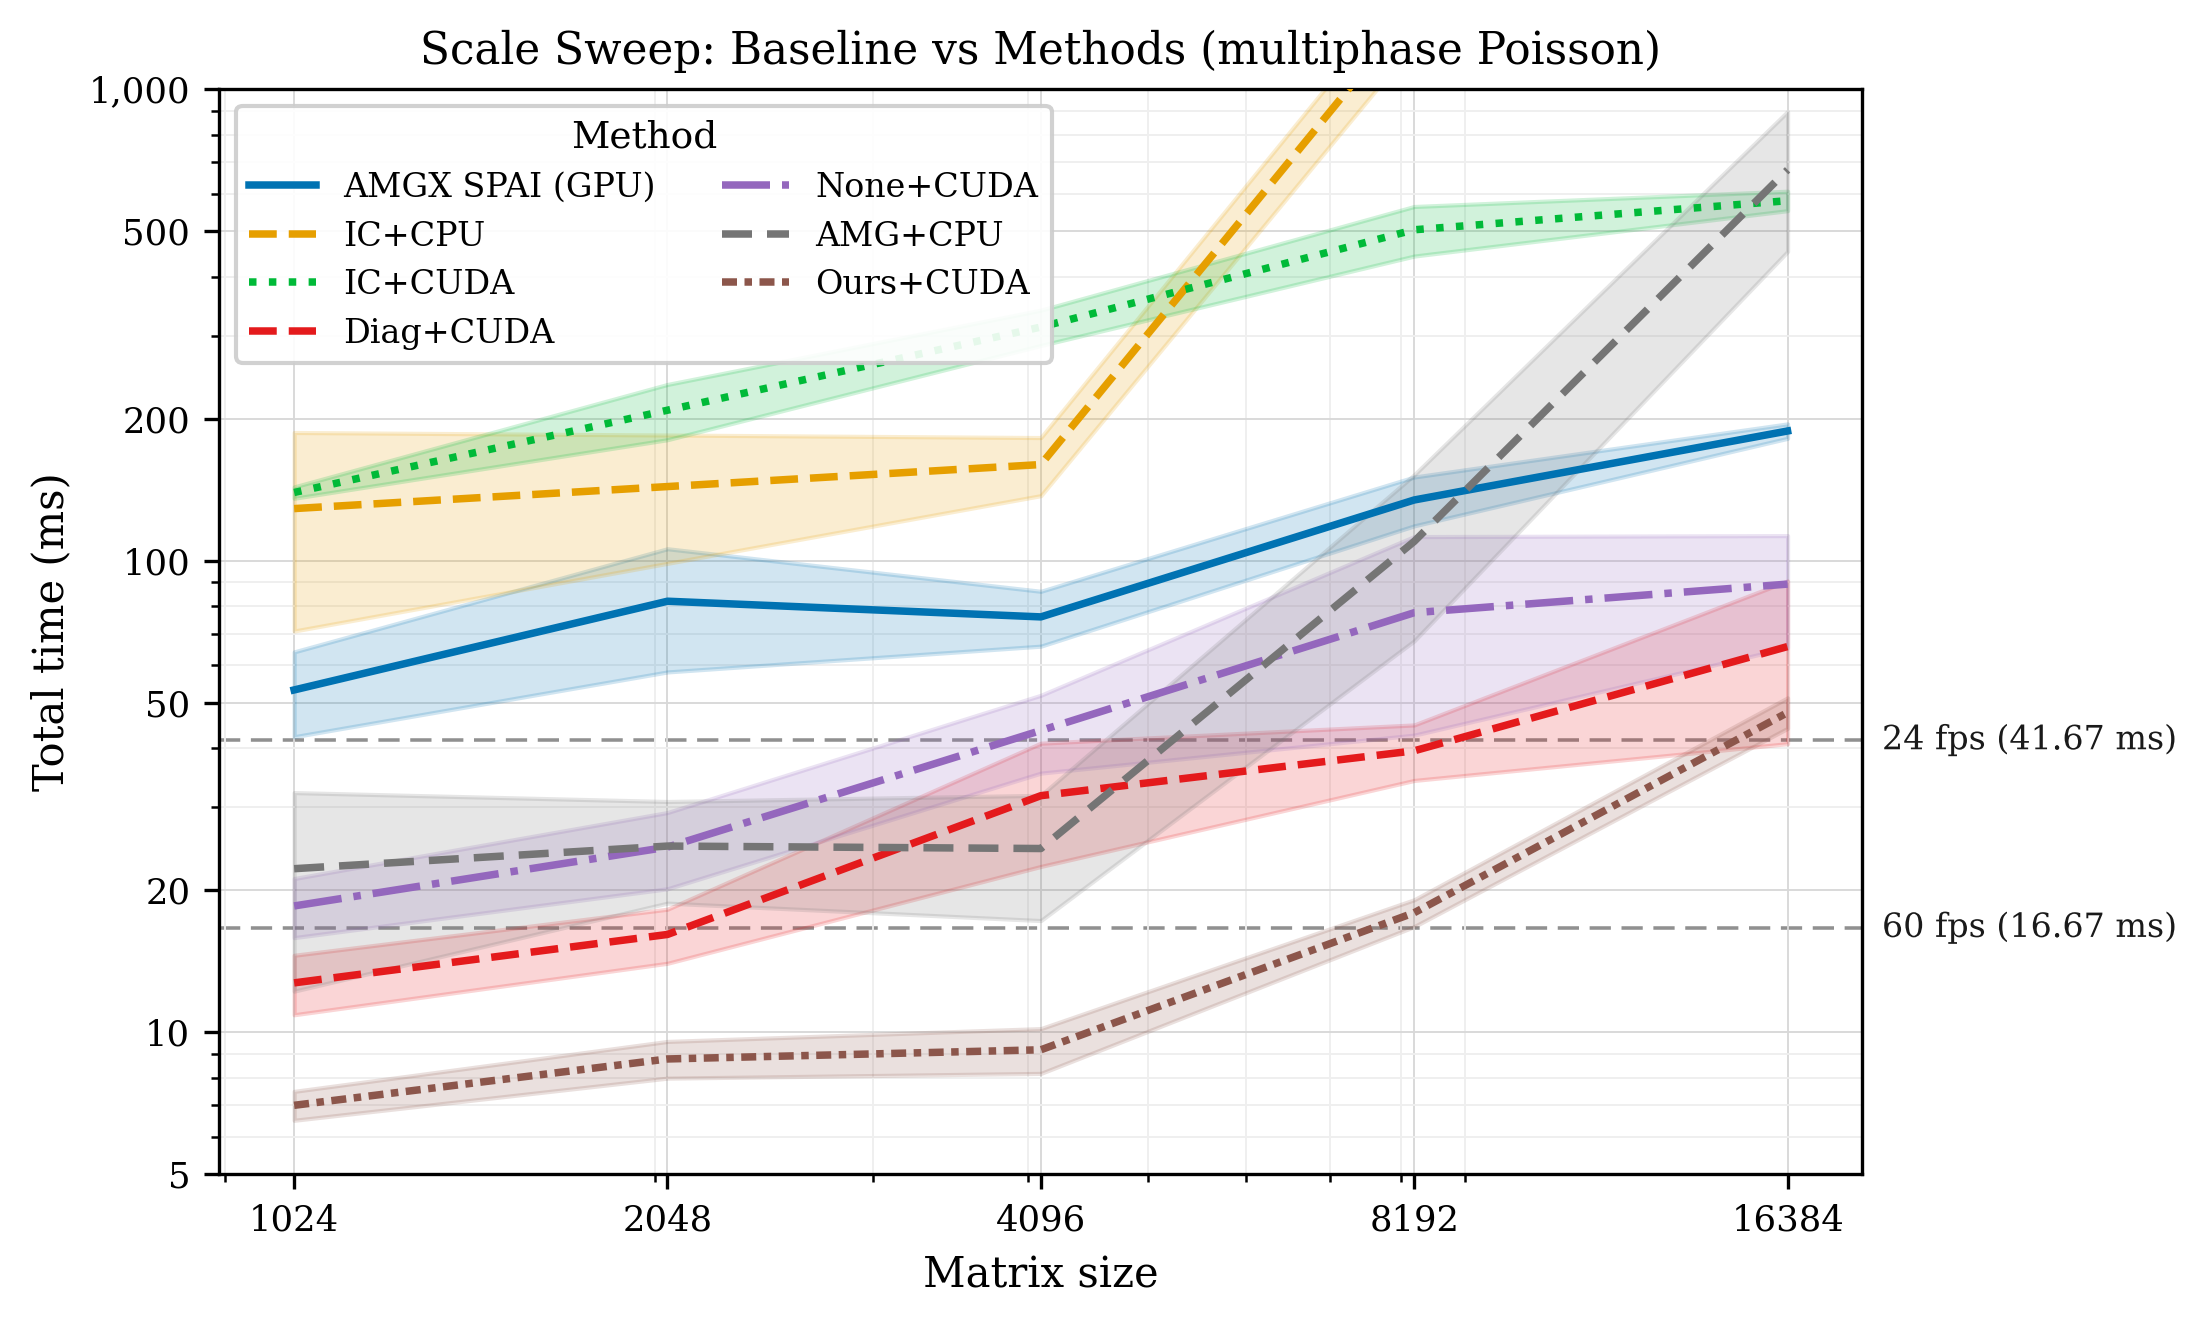
\includegraphics[width=0.85\textwidth]{scale_methods.png}
  \caption{End-to-end PCG solve time on the \textsf{multiphase\_v2} benchmark across five
  problem sizes, $20$ frames per scale (mean $\pm 1\sigma$ band; relative residual
  tolerance $10^{-8}$). Dashed grey lines mark the $24$\,fps and $60$\,fps interactive
  budgets. Our method is the only entry that fits within $60$\,fps for $N\!\le\!4{,}096$
  and within $24$\,fps for the entire range up to $N\!=\!16{,}384$; AMGX classical AMG and
  GPU IC-class (\textsc{multicolor\_dilu}) lie above $40$\,ms across all scales despite
  much lower iteration counts, because their per-iteration cost is dominated by
  unparallelizable triangular solves or V-cycle level synchronization.}
  \label{fig:scale_methods}
\end{figure*}

% --- TABLE: main performance table (Totals only; iter counts in supplementary) ---
\begin{table}[t]
\centering
\caption{Per-frame mean$\pm$std end-to-end PCG time (ms) on \textsf{multiphase\_v2} ($20$
frames per scale, $\mathrm{rtol}\!=\!10^{-8}$). ``$\dagger$''~=~CUDA Graph not supported.
Best per scale in \textbf{bold}. Iteration counts in Supplementary Material, Table~\ref{SX-tab:full_perf_table}.}
\label{tab:main:perf}
\footnotesize\setlength{\tabcolsep}{4pt}
\begin{tabular}{@{}l ccccc@{}}
\toprule
Method & $N{=}1024$ & $N{=}2048$ & $N{=}4096$ & $N{=}8192$ & $N{=}16384$ \\
\midrule
Unprec.~CG (GPU)             & $17.9\!\pm\!5.2$  & $24.0\!\pm\!8.9$   & $44.0\!\pm\!16.4$ & $70.6\!\pm\!68.8$ & $85.5\!\pm\!39.4$ \\
Jacobi (GPU)                 & $11.7\!\pm\!3.0$  & $15.8\!\pm\!4.2$   & $32.0\!\pm\!18.0$ & $38.8\!\pm\!10.5$ & $63.3\!\pm\!39.7$ \\
IC (CPU)$^\dagger$           &  $6.7\!\pm\!1.3$  & $25.8\!\pm\!5.4$   & $80.3\!\pm\!21.3$ & $711\!\pm\!207$   & $4{,}756\!\pm\!1177$ \\
IC / DILU (GPU)$^\dagger$    & $127.5\!\pm\!6.7$ & $191.7\!\pm\!11.3$ & $320\!\pm\!58$    & $450\!\pm\!84$    & $579\!\pm\!51$ \\
AMG (CPU)$^\dagger$          &  $9.7\!\pm\!2.8$  & $15.5\!\pm\!4.7$   & $17.0\!\pm\!9.4$  & $64.8\!\pm\!46.4$ & $271\!\pm\!164$ \\
AMG / AMGX (GPU)$^\dagger$   & $43.2\!\pm\!9.8$  & $56.9\!\pm\!14.4$  & $75.2\!\pm\!20.7$ & $117.7\!\pm\!4.1$ & $188.5\!\pm\!13.4$ \\
\textbf{Ours (GPU)}          & $\mathbf{6.5\!\pm\!0.8}$ & $\mathbf{7.7\!\pm\!1.3}$ & $\mathbf{9.0\!\pm\!1.9}$ & $\mathbf{18.1\!\pm\!2.4}$ & $\mathbf{46.5\!\pm\!6.9}$ \\
\midrule
\multicolumn{6}{l}{\emph{Speedup of Ours vs.\ each baseline at same scale:}} \\
~~vs.~Jacobi (GPU)           & $1.80\times$ & $2.05\times$ & $3.55\times$ & $2.14\times$ & $1.36\times$ \\
~~vs.~AMGX AMG (GPU)         & $6.63\times$ & $7.38\times$ & $8.35\times$ & $6.50\times$ & $4.05\times$ \\
~~vs.~AMGX DILU (GPU)        & $19.5\times$ & $24.8\times$ & $35.6\times$ & $24.8\times$ & $12.4\times$ \\
\bottomrule
\end{tabular}
\end{table}

\paragraph{Headline result.}
Figure~\ref{fig:scale_methods} and Table~\ref{tab:main:perf} present per-frame mean$\pm$std
solve time across $20$ test frames per scale. Three findings deserve emphasis. First, our
method is the only one that stays under the $60$\,fps interactive budget ($16.67$\,ms) for
$N\!\le\!4\,096$, and the only GPU method that stays under the $24$\,fps budget
($41.67$\,ms) at $N\!=\!16\,384$. Second, the closest contender at small scales is
GPU Jacobi (Diag), reflecting the fact that on small, well-conditioned blocks the
preconditioner-quality advantage barely matters: bandwidth dominates and Jacobi is as cheap
as you can be. The advantage of our method grows as the problem stiffens with scale ($N$
larger, contrast wider, more long-range coupling), peaks at $3.55\times$ over Jacobi at
$N\!=\!4\,096$, and shrinks to $1.36\times$ at $N\!=\!16\,384$ because our PCG iteration
count grows with $N$ ($50\!\to\!386$) while Jacobi's also does---both are $\Theta(N)$ per
iteration, and our absolute advantage at large $N$ comes from a $\sim\!4\!\times$ smaller
iteration count rather than from per-iteration speed. Third, the IC and AMG baselines
\emph{do} achieve very low iteration counts ($30$--$40$ for DILU, $1$--$3$ for AMG), but
their per-iteration cost is dominated by sequential triangular solves and level-by-level
V-cycle synchronization that map poorly onto the GPU---confirming the architectural
argument from Section~\ref{sec:application} (Table~\ref{tab:apply_complexity}).

\paragraph{Variance.}
Standard deviations track condition number, not problem size. Unpreconditioned CG has
$\sigma/\mu\!\approx\!50$--$100\%$ at $N\!\ge\!8\,192$ because individual frames span the
full $[5,100]$ contrast range; Jacobi shows similar relative spread; AMG-CPU spread is
extreme at $N\!=\!16\,384$ ($164$\,ms on $271$\,ms mean) because PyAMG's setup time scales
nonlinearly with the number of strong connections under high contrast. Our method's
$\sigma/\mu$ is the lowest among all converging methods at every scale ($\le\!21\%$
even at $N\!=\!16\,384$), indicating that the data-driven prior trained on the same
distribution is robust to the per-frame variation that breaks classical fixed-pattern
preconditioners.

% --- FIGURE: scalability (deferred until plot is generated) ---
% \begin{figure}[t]
%   \centering
%   \includegraphics[width=\linewidth]{figures/scalability.pdf}
%   \caption{Scalability of total solve time (Setup $+$ PCG) versus $N$ on the multiphase
%     benchmark, log--log axes. Dashed reference line indicates $O(N)$ slope. Error bars show
%     95\% confidence intervals over $[\cdot]$ test frames.}
%   \label{fig:scalability}
% \end{figure}

% --- FIGURE: convergence histories (deferred until data is available) ---
% \begin{figure}[t]
%   \centering
%   \includegraphics[width=\linewidth]{figures/convergence_histories.pdf}
%   \caption{Relative residual $\|A\mathbf{x}-\mathbf{b}\|/\|\mathbf{b}\|$ versus PCG iteration
%     on representative test frames at $N=8\,192$.}
%   \label{fig:convergence}
% \end{figure}

% ---------------------------------------------------------------------------
\subsection{Training Dynamics}
\label{sec:results:training}
% ---------------------------------------------------------------------------

% --- FIGURE: training dynamics (placed on a figures-only end page per SIGGRAPH Asia rules) ---
\begin{figure*}[p]
  \centering
  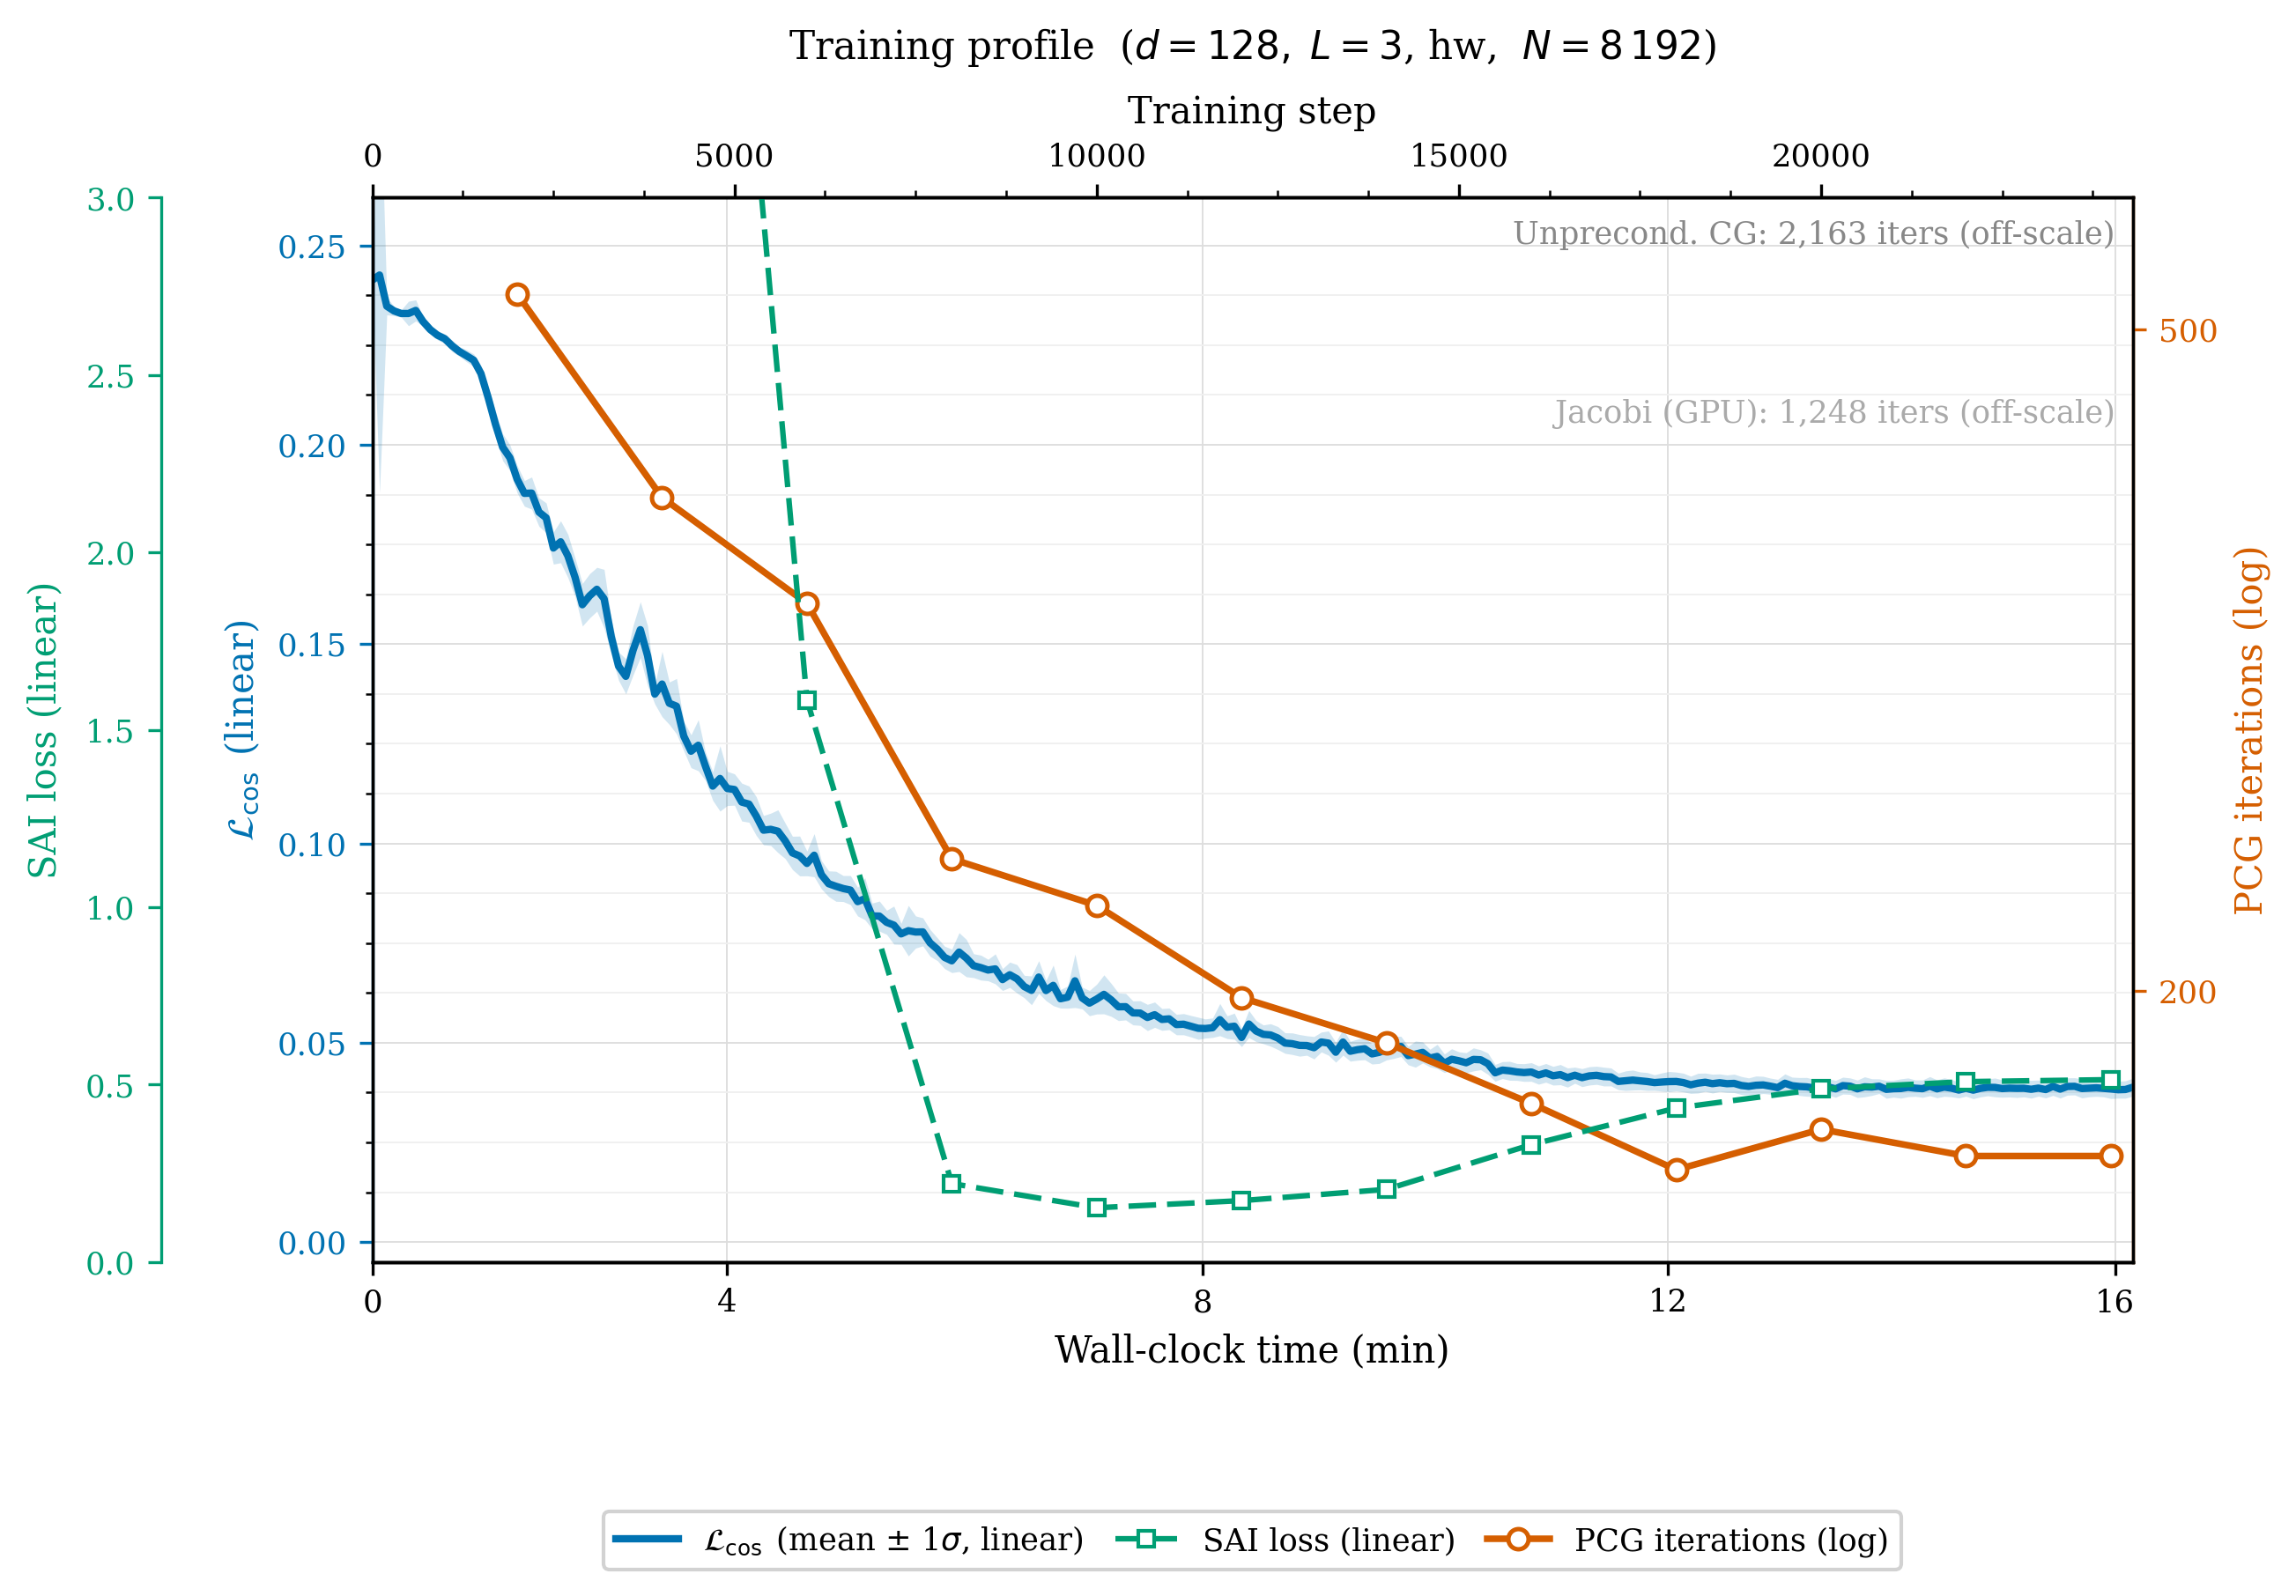
\includegraphics[width=0.7\textwidth]{training.png}
  \caption{Training profile of the configuration used in Table~\ref{tab:main:perf}
    ($N\!=\!8\,192$, $d\!=\!128$, $n_l\!=\!3$, highways). Blue: $\mathcal{L}_{\cos}$ on
    the training set (mean $\pm 1\sigma$, last 100 steps). Green dashed: SAI
    loss~\cite{Yang2025sparse} computed on a held-out validation frame at the same
    checkpoints (\emph{not} used for training). Orange: PCG iteration count to
    $\mathrm{rtol}\!=\!10^{-8}$ on that frame, log scale. Top axis: wall-clock minutes.
    Horizontal grey lines: unpreconditioned CG and Jacobi GPU baselines.}
  \label{fig:training:dynamics}
\end{figure*}

Figure~\ref{fig:training:dynamics} provides our clearest empirical evidence for the design
rationale of $\mathcal{L}_{\cos}$. Total wall-clock training time on a single GPU is
$16.2$\,min for $24\,300$ optimizer steps; the model beats GPU Jacobi by step
$\sim\!2{,}000$ ($\sim\!1.3$\,min) and drops under $200$ PCG iterations by step
$\sim\!12{,}000$ ($\sim\!8$\,min). The structural finding is in the relationship
\emph{between} the three curves. Up to step $\sim\!8\,000$, all three quantities decrease
together. After that, the SAI loss plateaus and then \emph{rises}, from $\sim\!10^{-3}$
at step $10\,000$ to $\sim\!0.5$ by step $24\,000$, even as $\mathcal{L}_{\cos}$ continues
to decrease smoothly and PCG iteration count continues to fall in lockstep with it. The
model is moving the eigenvalues of $MA$ \emph{away} from $\lambda\!=\!\|A\|$ in pointwise
terms, but \emph{toward} a tighter relative cluster wherever that turns out to be---the
exact behavior we predicted analytically in Section~\ref{sec:training:loss}, and the
single strongest argument for using a scale- and location-invariant cosine objective
rather than a Frobenius surrogate.

% ---------------------------------------------------------------------------
\subsection{Ablations}
\label{sec:ablation}
% ---------------------------------------------------------------------------

We ablate model width~$d$, transformer depth~$n_l$, and highway connections.  Each
configuration is trained independently to convergence on the same dataset.  Because not
every variant was evaluated at every problem size, the three groups in
Table~\ref{tab:ablation} report results at different scale sets; within each group all
variants share the same scale(s)---same held-out 20-frame test set, same convergence
criterion---and averages are taken across scales where more than one is available.
Section~\ref{sec:ablation:loss} and Figure~\ref{fig:training:dynamics} address the loss
objective separately.

% --- TABLE: ablation sweep ---
\begin{table}[t]
\centering
\caption{Hyperparameter ablations on \textsf{multiphase\_v2} ($\mathrm{rtol}\!=\!10^{-8}$,
$20$~frames per scale, neural preconditioner only).
\emph{Train}~=~wall-clock time to convergence (min);
\emph{Infer.}~=~preconditioner forward pass (ms);
\emph{Iters}~=~mean PCG iterations;
\emph{Total}~=~inference $+$ PCG solve (ms);
$\Delta$ solve time~=~fractional change in Total vs.\ the ``---'' row.}
\label{tab:ablation}
\footnotesize\setlength{\tabcolsep}{3.5pt}
\begin{tabular}{@{}l rr rr r@{}}
\toprule
Configuration & Train & Infer. & Iters & Total & $\Delta$ solve \\
              & (min) & (ms)   &       & (ms)  & time \\
\midrule
\multicolumn{6}{l}{\emph{Width} (avg.\ $N\!\in\!\{2048,4096,8192\}$):}\\
$d{=}64,\;n_l{=}3$, hw     &  9.5 & 3.0 & 147 & 15.4 & $+28\%$  \\
$d{=}128,\;n_l{=}3$, hw    & 10.7 & 3.1 & 105 & 12.0 & ---      \\
$d{=}256,\;n_l{=}3$, hw    & 12.3 & 3.2 & 191 & 19.3 & $+61\%$  \\
\midrule
\multicolumn{6}{l}{\emph{Depth} ($N\!=\!8192$):}\\
$d{=}128,\;n_l{=}1$, hw    &  6.1 & 1.3 & 421 & 36.9 & $+106\%$ \\
$d{=}128,\;n_l{=}2$, hw    &  9.6 & 2.3 & 218 & 20.8 & $+16\%$  \\
$d{=}128,\;n_l{=}3$, hw    & 16.2 & 3.4 & 168 & 17.9 & ---      \\
\midrule
\multicolumn{6}{l}{\emph{Highways} ($N\!=\!2048$):}\\
$d{=}128,\;n_l{=}3$, hw    &  6.0 & 3.3 &  66 &  8.8 & ---      \\
$d{=}128,\;n_l{=}3$, no-hw &  4.8 & 2.2 & 149 & 13.8 & $+58\%$  \\
\bottomrule
\end{tabular}
\end{table}

\subsubsection{Architecture}

\paragraph{Width.}
$d\!=\!256$ is competitive at small scales---fewer iterations than $d\!=\!128$ at
$N\!\in\!\{2048,4096\}$---but its iteration count nearly triples at $N\!=\!8\,192$
($454$ vs.\ $168$), so averaged across all three scales it is $61\%$ slower in total
solve time and $15\%$ more expensive to train.  A likely cause is that the larger
parameter count makes optimisation harder on the bigger graphs, where the training
signal per parameter is sparser and the loss landscape less well-conditioned; with
more careful tuning $d\!=\!256$ may well recover its small-scale advantage at larger
$N$.  $d\!=\!64$ is $28\%$ slower overall with only a modest training-time saving.
$d\!=\!128$ gave the most reliable behaviour across scales and was therefore chosen
as the default.

\paragraph{Depth.}
Depth has a larger and more monotone effect on both training cost and solve quality.
At $N\!=\!8\,192$, reducing from $n_l\!=\!3$ to $n_l\!=\!1$ cuts training time
$2.7\!\times$ ($16.2\!\to\!6.1$\,min) and inference cost $2.6\!\times$
($3.4\!\to\!1.3$\,ms), but increases PCG iterations $2.5\!\times$ and more than
doubles total solve time ($17.9\!\to\!36.9$\,ms)---the inference saving is consumed
many times over by extra CG work.  Depth $n_l\!=\!2$ still incurs a $16\%$
solve-time overhead despite only a $40\%$ training-time reduction.  The pattern
confirms that additional layers are needed to compose information routed through the
axial and global highway tokens.

\paragraph{Highways.}
Removing highway connections saves $20\%$ of training time ($6.0\!\to\!4.8$\,min) but
raises PCG iterations $2.3\!\times$ and total solve time $+58\%$ at $N\!=\!2\,048$,
and the solve-time penalty grows with problem size.  The highway buffers are the
mechanism by which independently processed transformer blocks exchange global spectral
context; without them, each block optimises a purely local factor with no awareness of
the bulk spectral shift required for effective long-range preconditioning.

\subsubsection{Loss}
\label{sec:ablation:loss}
We compare $\mathcal{L}_{\cos}$ against the SAI loss of~\cite{Yang2025sparse} on the same
architecture and training budget; Fig.~\ref{fig:loss:eigenvalues} shows the resulting
eigenvalue spectra of $MA$ at $N\!=\!1024$, the scale at which a full eigendecomposition is
tractable.  The training-curve argument from Section~\ref{sec:results:training} is confirmed
directly: SAI constrains eigenvalues to cluster near $\lambda\!=\!\|A\|$ and achieves a
$16\!\times$ condition-number reduction; $\mathcal{L}_{\cos}$ allows the cluster to settle
wherever the residual makes alignment easiest---here near $\lambda\!\approx\!0.08$---and
achieves a $68\!\times$ reduction, a $4.3\!\times$ better-conditioned system despite
identical architectures.  The bimodal cluster structure in both neural preconditioners
reflects the two-phase density contrast of the benchmark: light and heavy fluid regions
induce two eigenvalue groups whose relative spread sets the condition number.

\begin{figure}[t]
  \centering
  
\includegraphics[width=\linewidth]{solver_spectral_clustering.png}
  \caption{Eigenvalue spectra of $MA$ on a representative \textsf{multiphase\_v2} frame at
    $N\!=\!1024$ (full eigendecomposition, $y$-axis jittered for visibility).
    \emph{Top row}: unpreconditioned $A$ ($\tilde\kappa\!\approx\!5\!\times\!10^9$) and
    Jacobi ($1\!\times$ $\kappa$ reduction).
    \emph{Bottom row}: SAI-trained neural preconditioner ($16\!\times$ reduction,
    cluster anchored near $\lambda\!=\!\|A\|$ as required by the Frobenius objective) vs.\
    cosine-Hutchinson ($68\!\times$ reduction, cluster near $\lambda\!\approx\!0.08$,
    unconstrained by any location prior).  Both neural preconditioners share an identical
    architecture; the $4.3\!\times$ gap in $\kappa$ reduction is attributable entirely to
    the loss objective.}
  \label{fig:loss:eigenvalues}
\end{figure}

% ---------------------------------------------------------------------------
\subsection{Generalization, Precision, and Hardware Efficiency}
\label{sec:results:generalization}
% ---------------------------------------------------------------------------

We additionally evaluate three secondary axes whose detailed results we defer to the
supplementary material in the interest of space (Supplementary \S\ref{SX-supp:generalization}
and \S\ref{SX-supp:precision}):
(i)~\emph{Out-of-distribution generalization}---models trained at one scale evaluated at
larger and smaller $N$, and at contrast ratios outside the training range $[5,100]$;
(ii)~\emph{Precision sensitivity}---float32 vs.\ mixed-precision vs.\ float64 in the apply
path, with PCG scalar accumulators held at float64 throughout;
(iii)~\emph{Hardware efficiency}---achieved Tensor Core utilization and DRAM bandwidth
during apply, contrasted with the bandwidth-bound Jacobi and SpMV-bound IC kernels.
The pattern across all three is consistent with the headline result: as the problem class
moves further from the training distribution, our advantage over Jacobi narrows but
remains positive across the entire range we tested. % TODO: insert OOD speedup numbers when ready.

% ===========================================================================
\section{Limitations and Future Work}
\label{sec:limitations}
% ===========================================================================

Three limitations are worth flagging. (i) The $\mathcal{H}$-matrix partition is fixed by
the index ordering of $A$; discretizations with poor spatial locality after Morton/RCM
(e.g.\ irregular unstructured meshes) may have weaker low-rank structure on admissible
tiles. (ii) The partition is keyed to $N$ and $L$, so extreme rescaling
($\!\gtrsim\!4\times$ larger) currently requires retraining. (iii) Our preconditioner is
symmetric but not strictly SPD: the diagonal contribution is PSD, but the off-diagonal
contributions are symmetric and generally indefinite. PCG converges robustly in
experiments, but flexible GMRES~\cite{saad1993flexible} would lift this assumption and
extend to non-symmetric systems---a direction we leave to future work along with
input-adaptive partitioning that preserves single-graph capture. To summarize: a fixed
$\mathcal{H}$-matrix partition combined with a coarse-rank transformer-emitted off-diagonal
stream and a $\Theta(N)$ allocation-free apply path yields the only method we evaluate that
fits an interactive-fps budget across $1{,}024$--$16{,}384$ unknowns on stiff multiphase
pressure-Poisson.

\section*{Acknowledgments}
Omitted for anonymous review.

\bibliographystyle{ACM-Reference-Format}
\bibliography{references}

\end{document}
